\documentclass[a4paper,12pt]{book}

%\usepackage[T1]{newtxtext} % carattere times new roman
\usepackage{step}

%\usepackage{fontspec}
%\setmainfont{Times New Roman} % carattere times new roman
\usepackage[italian]{babel}
\linespread{1.5}

\setlength{\parindent}{0em} % indentazine paragrafo nulla
\usepackage{ragged2e} % testo giustificato

\usepackage{graphicx}
\usepackage[hidelinks]{hyperref} % link nel documento
\usepackage{float} % [H] in immagini

\usepackage{color}
\usepackage{listings} % inserire codice

\lstset{ %
    tabsize = 3, %% set tab space width
    showstringspaces = false, %% prevent space marking in strings, string is defined as the text that is generally printed directly to the console
    numbers = left, %% display line numbers on the left
    commentstyle = \color{green}, %% set comment color
    keywordstyle = \color{blue}, %% set keyword color
    stringstyle = \color{red}, %% set string color
    rulecolor = \color{black}, %% set frame color to avoid being affected by text color
    basicstyle = \small \ttfamily , %% set listing font and size
    breaklines = true, %% enable line breaking
    numberstyle = \tiny,
}

\usepackage{longtable} % tabelle multipagina
\usepackage{dirtree} % creare struttura progetto

\usepackage{fancyhdr} % numerazione pagine
\pagestyle{fancy}
\fancyhead{}
\fancyhead[LO]{\rightmark}
\fancyhead[RE]{\leftmark}

\usepackage[left=3cm, right=3cm, bottom=3cm, top=3cm]{geometry}

\renewcommand\lstlistlistingname{Elenco del codice} % Nome personalizzato listings

\usepackage{biblatex} % bibliografia
\addbibresource{chapters/biblio.bib}

\usepackage[acronym]{glossaries}
\makeglossaries
\loadglsentries{chapters/gloss}



\begin{document}

%%%%%%%%%%%%%%%% PRIMA PAGINA %%%%%%%%%%%%%%%%
\begin{titlepage}
\begin{center}

\includegraphics[height=2.22cm]{images/unipd_800_logotipo_sigillo.pdf}  \hfill 
\includegraphics[height=2.22cm]{images/dei_sigillo_logotipe.pdf}  \\

\vspace{2cm}
\textsc{\LARGE Università degli Studi di Padova}\\
\vspace{0.45cm}
\textsc{\large Dipartimento di Ingegneria dell'Informazione}\\
\vspace{0.4cm}
\textsc{\large Corso di Laurea Triennale in}\\
\textsc{\large Ingegneria Informatica}\\
\vfill
% Title
{ \LARGE \bfseries Utilizzo del framework Spring e del broker di messaggi RabbitMQ in una applicazione web per il corporate social networking}\\
\vfill
\textit{\large Relatore:} \hfill \textit{\large Laureando:}\\
\textsc{\large Prof. Fantozzi Carlo} \hfill \textsc{Luisetto Federico}\\
\hfill \textsc{1187521}\\

\vfill
% fondo pagina
{\large Anno Accademico 2021/2022}\\
{\large Data di laurea 07/03/2022}
\end{center}
\end{titlepage}

%%%%%%%%%%%%%%%% FINE PRIMA PAGINA %%%%%%%%%%%%%%%%

\thispagestyle{empty} %pagina bianca dopo il titolo
\cleardoublepage

% numerazione romana per l'indice, il sommario e i ringraziamenti
\pagenumbering{roman}
\thispagestyle{empty}

\clearpage{\pagestyle{plain}\cleardoublepage}
\pdfbookmark{\contentsname}{abs}
%definisco il layout della pagina
\def\changemargin#1#2{\list{}{\rightmargin#2\leftmargin#1}\item[]}
\let\endchangemargin=\endlist 

%Genero l'ambiente per il sommario
\newcommand\summaryname{Sommario}
\newenvironment{Sommario}%
    {\begin{center}%
    \bfseries{\summaryname} \end{center}}
    
\begin{Sommario}
\begin{changemargin}{1cm}{1cm}
Il presente documento descrive il mio lavoro svolto durante il periodo di tirocinio, della durata di circa duecentocinquanta ore, presso l'azienda Sync Lab.\\
Il lavoro di tirocinio si inserisce in un progetto, denominato Challenginator, che consiste nello sviluppo di un'applicazione web per la gestione di sfide tra colleghi.\\
Gli obiettivi di questo tirocinio erano molteplici. In primo luogo era richiesto lo studio teorico delle applicazioni a microservizi, del 
framework Spring e del broker RabbitMQ. In secondo luogo era richiesta l'implementazione del servizio di notifica tramite e-mail di Challenginator.
Infine era richiesto un meccanismo di log per l'applicazione web, così da facilitare il debugging in caso di future modifiche a quest'ultima.
\end{changemargin}
\end{Sommario}

% indice
\clearpage{\pagestyle{plain}\cleardoublepage}
\pdfbookmark{\contentsname}{toc}
\tableofcontents
% lista figure
\clearpage{\pagestyle{plain}\cleardoublepage}
%\pdfbookmark{\listfigurename}{lof}
\listoffigures
% lista tabelle
\clearpage{\pagestyle{plain}\cleardoublepage}
%\pdfbookmark{\listtablename}{lot}
\listoftables
% lista codice
\clearpage{\pagestyle{plain}\cleardoublepage}
%\pdfbookmark{\listtablename}{lol}
\lstlistoflistings
% numerazione araba per i capitoli
\clearpage{\pagestyle{plain}\cleardoublepage} 
\pagenumbering{arabic}

%%%%%%%%%%%%%%%% CORPO DOCUMENTO %%%%%%%%%%%%%%%%
\chapter{Introduzione}\label{introduzione}

\section{L'azienda}\label{azienda}

\begin{figure}[H]
    \centering
    
\includegraphics{images/logo-synclab.pdf}
    \caption{Logo azienda Sync Lab. Fonte: SyncLab}
\end{figure}

Sync Lab \cite{synclab} nasce come \textit{software house} a Napoli nel 2002. Rapidamente cresciuta nel mercato dell' \acrshort{ict} ora è un \textit{system integrator} che conta 6 sedi in Italia e più di 300 dipendenti. 
\\
L'azienda propone innovativi prodotti software che spaziano in diversi settori: \acrshort{gdpr}, Big Data, Cloud Computing, \acrshort{iot}, Mobile e Cyber Security. Grazie alla vasta gamma di soluzioni offerte Sync Lab lavora in diversi mercati, quali Sanità, Industria, Energia, Finanza e Trasporti \& Logistica.

\section{Challenginator}\label{intro_challenginator}

Challenginator \ref{challenginator} è un progetto interno all'azienda ideato per permettere ai propri dipendenti di sfidarsi l'un l'altro in attività inerenti alla vita lavorativa. L'intento è quello di contribuire alla crescita personale del singolo, cercando di migliorare le dinamiche lavorative.\\
L'idea di base è semplice: un collega ne sfida un altro in un'attività (ad esempio timbrare in orario, ordinare quotidianamente la scrivania etc.) e un superiore supervisionerà l'operato, giudicando lo sfidato.\\
Per l'implementazione è stato utilizzato il linguaggio \Gls{spring} \ref{spring} data la sua leggerezza e modularità; grazie a quest'ultima è stato possibile selezionare solo le componenti necessarie per il progetto. Tra queste troviamo \textit{Data JPA} per la comunicazione con il database, \textit{Data REST} per lo scambio di dati mediante chiamate \acrshort{rest} e \textit{Cloud} per aggiungere un servizio atto all'individuazione delle componenti (microservizi) dell'applicazione.\\ Il \Gls{dbms} scelto per salvare in modo persistente i dati è \Gls{postgresql}, dato che si è lavorato con database relazionali.\\ L'invio delle email ed il servizio di log sono affidati al broker \Gls{rabbitmq}, preferito a Kafka per i motivi descritti nella Sezione \ref{rabbitmq}.\\ Per la scrittura, la manutenzione ed il testing del progetto è stato utilizzato dell'altro software, descritto nello specifico nella Sezione \ref{software}.\\
Il mio contributo a questo progetto è costituito dall'implementazione, assieme ad un collega, del servizio di notifica e l'implementazione, autonoma, del servizio di logging.
\chapter{Metodologie e tecnologie}\label{teoria}

In questo capitolo descriverò gli strumenti utilizzati per la realizzazione ed il testing del progetto. Tra di essi mi soffermerò in particolare sul \textit{framework} \gls{spring} (e relativi moduli derivati), il broker \gls{rabbitmq} e l'architettura a microservizi dato che sono stati i principali ambiti di studio nel periodo di tirocinio.

%%%%%%%%%%  ARCHITETTURA A MICROSERVIZI %%%%%%%%%%
\section{Architettura a Microservizi}

\begin{figure}[H]
    \centering
    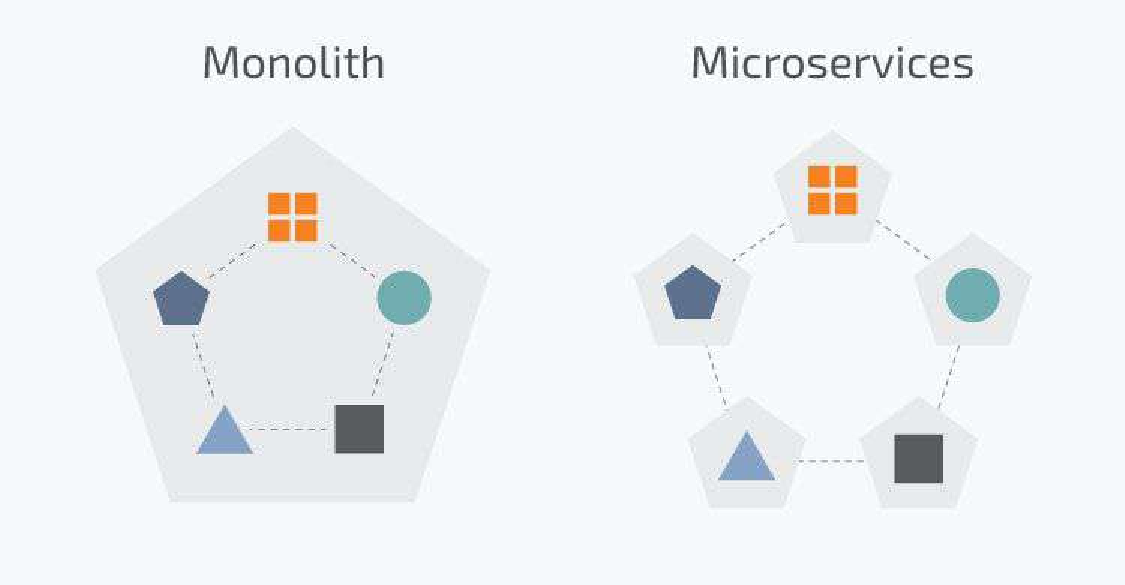
\includegraphics[width=11cm, height=6cm]{images/monoVSmicro.pdf}
    \caption{Architettura monolitica vs microservizi. Fonte: N-iX}
\end{figure}

Nel mondo della programmazione una delle nuove tendenze è l'adozione dell'architettura a microservizi per la creazione di applicazioni \cite{monomicro}. L'approccio a microservizi offre infatti vantaggi tangibili, tra cui un aumento della scalabilità, della flessibilità e dell'agilità. Molti leader tecnologici hanno effettuato con successo il passaggio dall'architettura monolitica ai microservizi, e ad ora molte aziende considerano di seguire questo esempio come il modo più efficiente per la crescita del business.\\
Dal canto suo l'approccio monolitico è un modello predefinito per la creazione di un'applicazione software. Tuttavia la sua popolarità sta diminuendo dato che questo tipo di architettura pone una serie di sfide associate, quali una grossa mole di codice, la difficoltà nell'adozione di una nuova tecnologia e dell'implementazione di modifiche.

\subsection{Monolitica vs. Microservizi}
%%%%%%%%%%  ARCHITETTURA MONOLITICA %%%%%%%%%%
\begin{flushleft}
\textbf{{\large Architettura Monolitica}}
\end{flushleft}

L'architettura monolitica è considerata la via tradizionale nella costruzione delle applicazioni. Un'applicazione monolitica è costituita da una singola ed indivisibile unità dove vengono gestite tutte le operazioni. Tra queste possiamo trovare l'interfaccia grafica atta alla comunicazione con l'utente e la comunicazione/gestione del database. Di prassi l'architettura monolitica è caratterizzata da una grande mole di codice e da mancanza di modularità. Se è necessario effettuare un aggiornamento o cambiare qualcosa, i programmatori dovranno accedere allo stesso codice, modificando l'intera applicazione.

\begin{figure}[H]
    \centering
    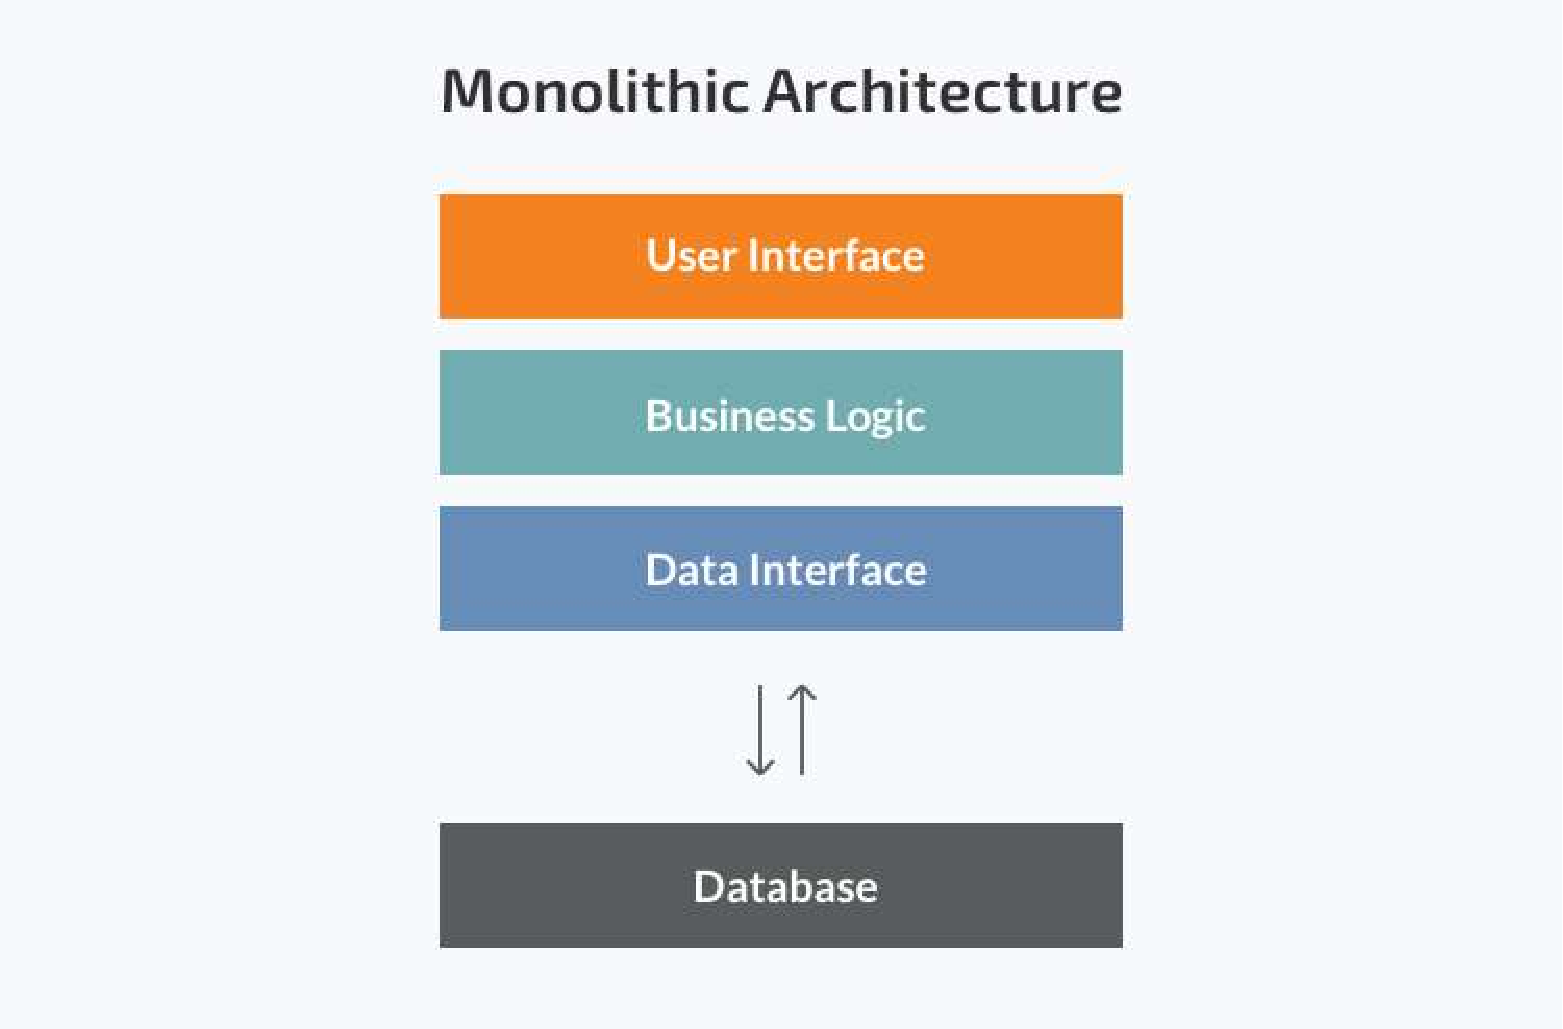
\includegraphics[width=10cm, height=6cm]{images/mono.pdf}
    \caption{Architettura monolitica. Fonte: N-iX}
\end{figure}

I punti di forza di questo tipo di architettura sono la semplicità di sviluppo, derivante dal fatto che il modello monolitico è uno standard per creare applicazioni, e di distribuzione, la riduzione dei problemi trasversali quali il \textit{logging}, il \textit{caching} ed il monitoraggio delle prestazioni. Infine il \textit{debugging} ed il \textit{testing} sono più semplici dato che riguardano una singola unità indivisibile.\\
I punti di debolezza sono principalmente legati alla gestione del codice nel tempo. Mano a mano che l'applicazione si arricchisce di nuove funzionalità diventa difficile la comprensione d'insieme.

\begin{table}[H]
    \centering
    \begin{tabular}{ |c|c| }
        \hline
        Pro & Contro \\
        \hline
        Meno problemi trasversali & Difficoltà di comprensione \\
        Semplicità debugging e testing & Difficoltà nella manutenzione \\
        Semplicità di sviluppo & Nessuna scalabilità di componenti \\
        Semplicità di distribuzione & Problematica nuove tecnologie \\
        \hline
    \end{tabular}
    \caption{Pro e contro di una architettura monolitica}
\end{table}
%%%%%%%%%%  ARCHITETTURA A MICROSERVIZI %%%%%%%%%%
\begin{flushleft}
\textbf{{\large Architettura a Microservizi}}
\end{flushleft}

Mentre un'applicazione monolitica è una singola indivisibile unità, l'architettura a microservizi suddivide l'applicazione in una raccolta di unità indipedenti più piccole. Queste unità eseguono ogni processo dell'applicazione come un servizio separato, così ognuno di questi servizi può avere una propria logica ed un proprio database.\\
All'interno di un'architettura a microservizi l'intero applicativo è suddiviso in moduli distribuiti in modo indipendente che comunicano tra loro attraverso le \Gls{api}. Ogni servizio può essere aggiornato, distribuito e ridimensionato in modo indipendente.

\begin{figure}[H]
    \centering
    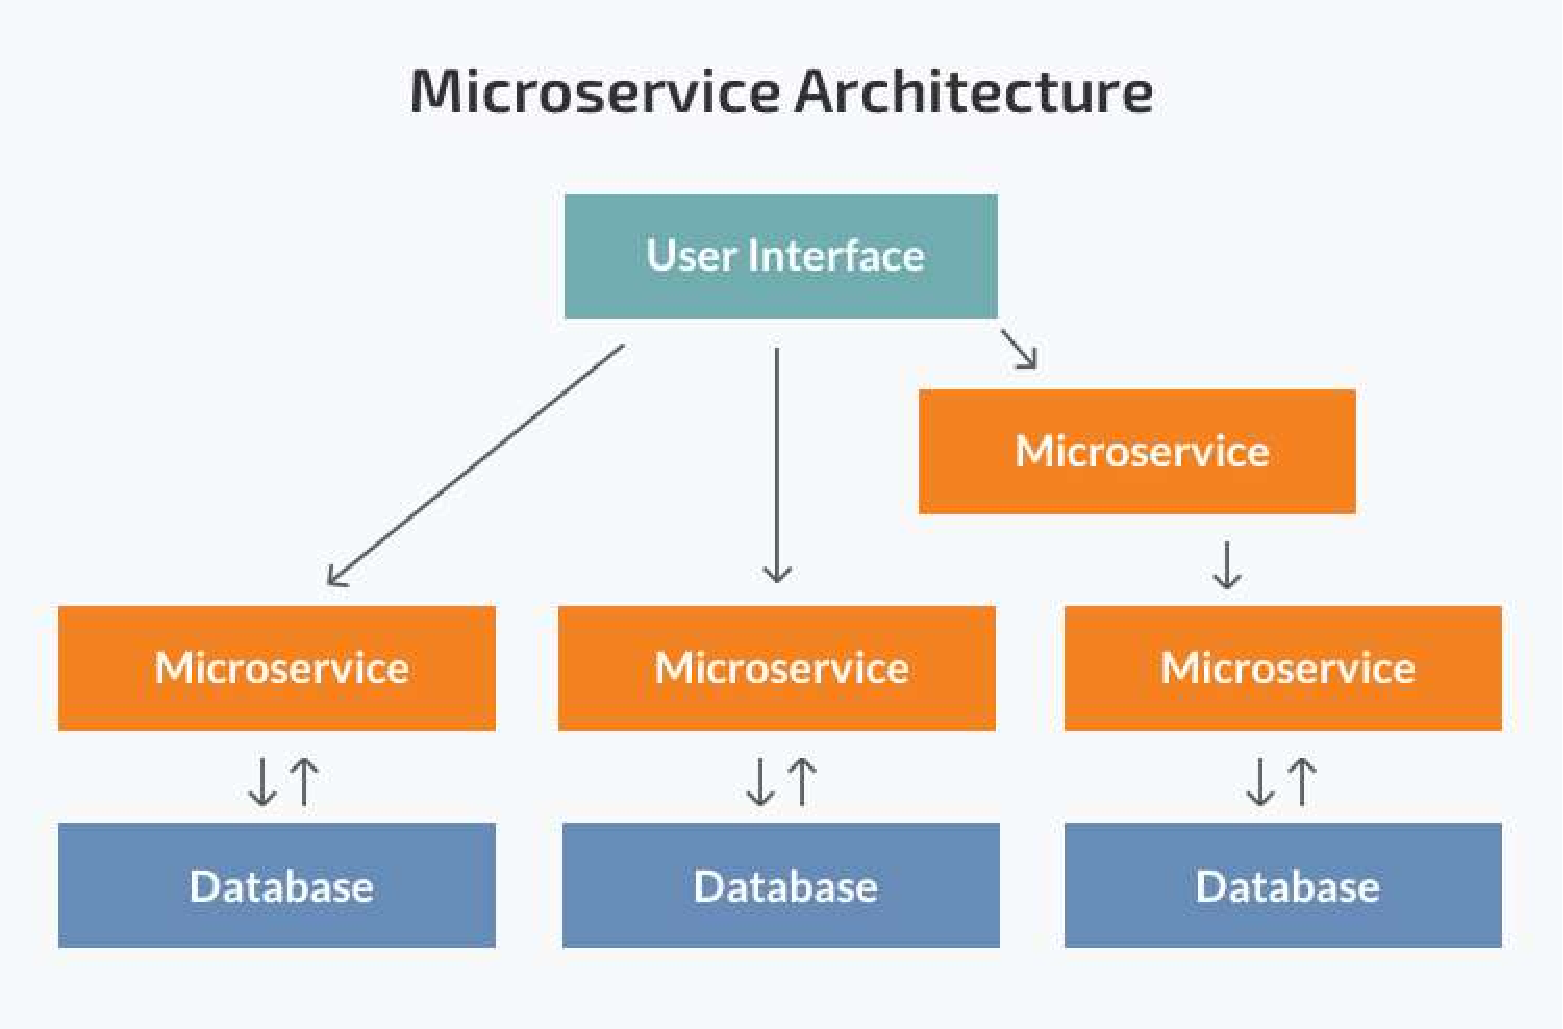
\includegraphics[width=10cm, height=6cm]{images/micro.pdf}
    \caption{Architettura a microservizi. Fonte: N-iX}
\end{figure}

I punti di forza di questo tipo di architettura sono l'indipendenza delle componenti, che permette l'implementazione e l'aggiornamento del singolo modulo; da questo deriva anche una migliore scalabilità ed il confinamento dei bug, dato che il malfunzionamento di un servizio non comporta l'interruzione di tutta l'applicazione. La divisione dei vari servizi permette una migliore e più semplice comprensione dell'applicazione ed una maggiore flessibilità nella scelta delle tecnologie.\\
I punti di debolezza riguardano la complessità di realizzazione e di \textit{testing} di un'applicazione con questa architettura, l'incremento di problemi trasversali nell'implementazione e la difficoltà di distribuzione, data l'interconnessione di più moduli indipendenti.

\begin{table}[H]
    \centering
    \begin{tabular}{ |c|c| }
        \hline
        Pro & Contro \\
        \hline
        Indipendenza delle componenti & Complessità aggiuntiva \\
        Facilità di comprensione & Difficoltà di distribuzione \\
        Migliore scalabilità & Problematiche trasversali \\
        Flessibilità nelle tecnologie & Testing difficoltoso \\
        \hline
    \end{tabular}
    \caption{Pro e contro di una architettura a microservizi}
\end{table}

\subsection{Componenti microservizi}

%%%%%%%%%%  API GATEWAY %%%%%%%%%%  
\begin{flushleft}
\textbf{{\large API Gateway}}
\end{flushleft}

\begin{figure}[H]
    \centering
    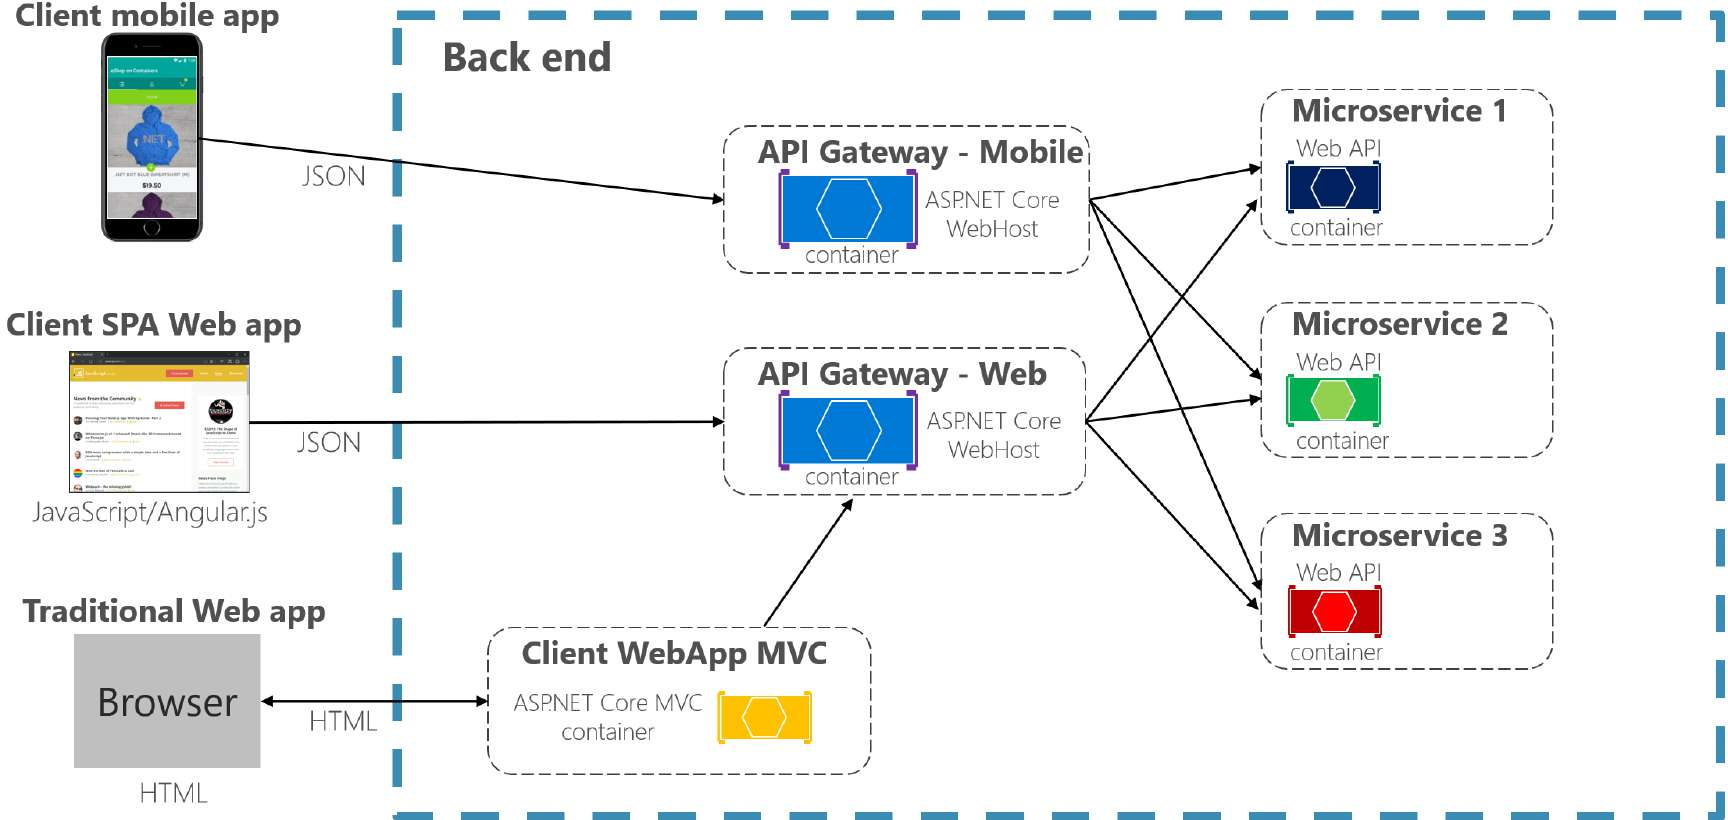
\includegraphics[width=13cm, height=8cm]{images/api-gateway.pdf}
    \caption{Servizio API Gateway. Fonte: Microsoft}
    \label{fig:apigat}
\end{figure}

%%%%%%%%%%  Circuit Breaker %%%%%%%%%%  
\begin{flushleft}
\textbf{{\large Circuit Breaker}}
\end{flushleft}

Il \textit{circuit breaker} è un modello di progettazione utilizzato nell'architettura a microservizi. I vari servizi per interagire tra loro si scambiano dati mediante richieste attraverso la rete. Durante questo scambio di informazioni è possibile che un servizio sia inattivo, per una connessione lenta, un timeout o un'indisponibilità temporanea. La soluzione migliore è far richiesta nuovamente a quel servizio, però se il problema è grave e quest'ultimo non è a disposizione per lungo tempo si può incorrere nell'eventualità in cui le chiamate a quel servizio saturino la rete, compromettendo le prestazioni e l'esperienza utente. Per ovviare a queste problematiche si utilizza il \gls{pattern} \textit{circuit breaker}: quando il numero di guasti di un servizio supera una determinata soglia l'interruttore va in stato \textit{open} per un periodo di \textit{timeout}, ritornando un errore al servizio chiamate ad ogni nuova chiamata. Trascorso questo lasso temporale l'interruttore va in stato \textit{half-open}, consentendo il passaggio di un limitato numero di richieste di richieste di test. Se queste ultime avranno esito positivo l'interruttore andrà in stato \textit{closed} e riprende il normale funzionamento. In caso contrario il periodo di \textit{timeout} ricomincia.

Un API Gateway funge da "porta d'ingresso" per accedere ai vari microservizi da un singolo punto di accesso ed anche da \textit{proxy} inverso dato che indirizza le richieste dai client ai servizi. Questo servizio sta nel mezzo tra le applicazioni ed i microservizi così non è necessario esporre i singoli applicativi, aumentando così la sicurezza. In figura \ref{fig:apigat} si nota che solitamente si utilizza più di un API Gateway così da non avere un aggregatore monolitico (che violerebbe l'autonomia dei microservizi accoppiandoli tutti tra loro).

%%%%%%%%%%  Service Discovery e Service Registry    %%%%%%%%%%
\begin{flushleft}
\textbf{{\large Service Discovery e Service Registry}}
\end{flushleft}

\begin{figure}[H]
    \centering
    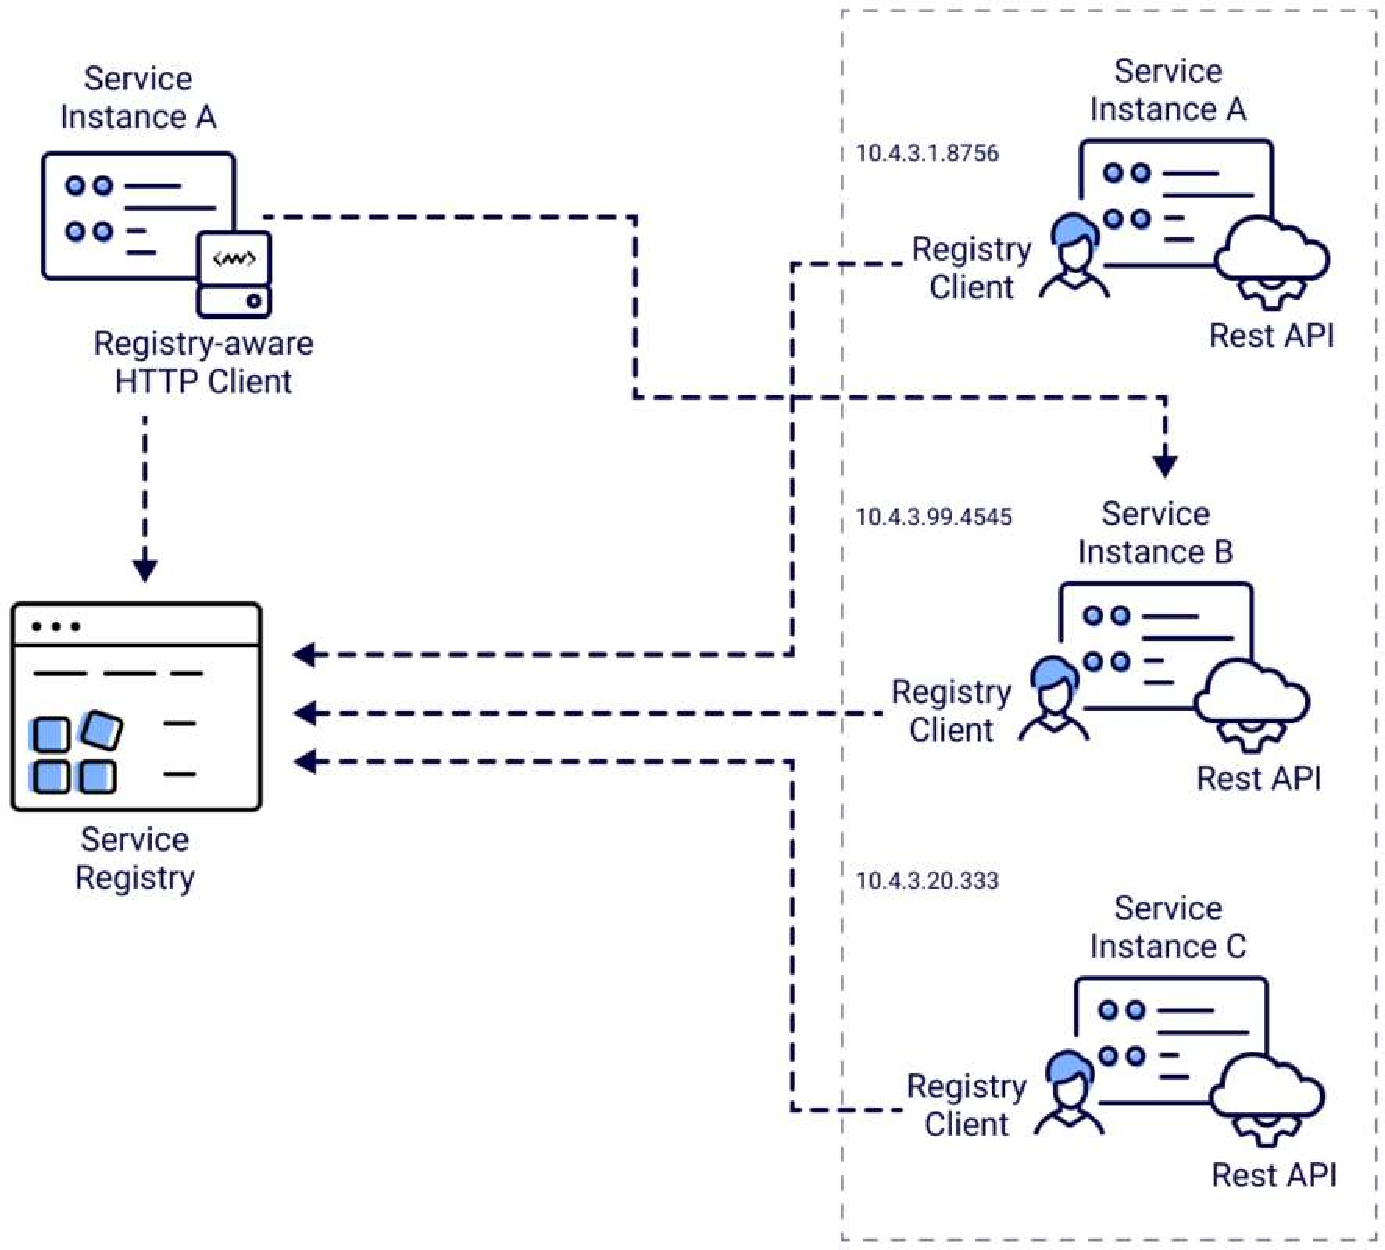
\includegraphics[width=12cm, height=9cm]{images/service-discovery.pdf}
    \caption{Schema del Service Discovery. Fonte: Middleware}
    \label{fig:servdisc}
\end{figure}

Il \textit{service discovery} è un protocollo di rete utilizzato per la rilevazione automatica di servizi e dispositivi in rete. In figura \ref{fig:servdisc} è rappresentato un \textit{service discovery} lato client come quello utilizzato nel progetto; in questo tipo di servizio il client deve ricercare il \textit{service registry} per poter individuare un servizio. Quindi il client seleziona un'istanza del servizio libera mediante un algoritmo di bilanciamento del carico.\\
Il \textit{service registry} è una componente fondamentale del \textit{service discovery}. Esso è costituito da un database contenente le locazioni di tutte le istanze dei servizi disponibili. I client possono salvare le locazioni ottenute dal \textit{service registry} nella cache, ma non devono appoggiarsi ai dati ottenuti per troppo tempo dato che quelle informazioni possono diventare velocemente obsolete.

%%%%%%%%%%  SPRING  %%%%%%%%%%
\section{Spring}\label{spring}
\Gls{spring} è un framework open source per lo sviluppo di applicazioni su piattaforma Java. Ad esso sono associati tanti altri progetti, modulari, che ne completano le funzionalità. Questi hanno nomi composti, come \textit{Spring Boot}, \textit{Spring Data} o \textit{Spring Security}. Seguirà ora un elenco dei componenti di questo framework da me utilizzati.

\begin{itemize}
    \item \textbf{Spring Boot}: questo modulo permette la creazione di una applicazione utilizzante il \textit{framework} \Gls{spring} pronta all'uso. Mediante \textit{Spring Inizializr}, \textit{Spring Boot} imposta i parametri dell'applicativo da creare (quali nome del progetto, il linguaggio utilizzato, i metadata del progetto ed il packaging) ed aiuta ad aggiungere le dipendenze necessarie tramite un checkbox.
    \item \textbf{Spring Data REST}: questo modulo permette la gestione dell'applicazione mediante chiamate \acrshort{rest} e la navigazione attraverso link.
    \item \textbf{Spring Data JPA}: questo modulo semplifica la comunicazione col database da parte dell'applicazione mediante \Gls{jpa}. Permette l'esecuzione di query, nonché l'impaginazione ed il controllo dei dati.
    \item \textbf{Spring REST Docs}: questo modulo è utile per la scrittura della documentazione progettuale e durante la fase testing. Utilizzando Postman \ref{postman}, mediante la chiamata GET \texttt{http://localhost:808x/v3/api-docs} (\textbf{x} indica un numero da 0 a 5, in base al microservizio da testare), si ha a disposizione una descrizione dei campi necessari per poter effettuare una chiamata POST o SET a quel microservizio.
    \item \textbf{Spring AMQP}: questo modulo è necessario per la corretta comunicazione dei microservizi col broker. Permette di inviare e ricevere messaggi e la dichiarazione di nuove \textit{queue}, \textit{exchange} e \textit{bindings}.
    \item \textbf{Spring Cloud Circuit Breaker}: questo modulo fornisce un'astrazione tra le diverse implementazioni dei \textit{circuit breaker}.
    \item \textbf{Spring Cloud Gateway}: questo modulo permette la creazione di un \acrshort{api} Gateway che fornisce un semplice ma efficace modo per instradare le chiamate dell'utente ai vari microservizi.
    \item \textbf{Spring Cloud Netflix}: questo modulo introduce nel progetto il \textit{service discovery} Eureka
    \item \textbf{Spring Security}: questo modulo è un framework di autenticazione e controllo accessi potente e altamente personalizzabile. È lo standard de facto per la protezione delle applicazioni basate su Spring.
\end{itemize}
%%%%%%%%%%  RABBITMQ    %%%%%%%%%%
\section{RabbitMQ}\label{rabbitmq}

\Gls{rabbitmq} è un broker di messaggi che utilizza il protocollo \acrshort{amqp} per svolgere le sue funzioni. \acrshort{amqp} è uno standard aperto che definisce un protocollo a livello applicativo per il \textit{message-oriented middleware}; questo standard è definito in modo tale da garantire funzionalità di messaggistica, accodamento e \textit{routing}, affidabilità e sicurezza \cite{amqprab}. Un broker di messaggi è una tecnologia che si fa carico della convalida, della trasformazione e del corretto indirizzamento dei messaggi. Questo strumento media la comunicazione tra le applicazioni permettendo la comunicazione attraverso lo scambio di messaggi, che possono includere qualsiasi tipo di informazione.\\
Le componenti di \Gls{rabbitmq} sono le seguenti
\begin{itemize}
    \item \textit{Publisher}: entità che comunica col broker per inviare un messaggio.
    \item \textit{Consumer}: entità che riceve un messaggio dal broker.
    \item \textit{Queue}: entità dove i messaggi sono custoditi prima dell'invio al consumer. Il legame tra \textit{queue} ed \textit{exchange} è chiamato \textit{binding}.
    \item \textit{Exchange}: entità che riceve i messaggi dal \textit{publisher} e li accoda in una o più \textit{queue}. Ci sono più tipi di \textit{exchange}.
    \begin{itemize}
        \item \textit{Fanout} accoda tutti i messaggi in tutte le \textit{queue} che conosce.
        \item \textit{Direct} accoda il messaggio alle code la cui chiave di associazione corrisponde esattamente alla \textit{routing key} del messaggio.
        \item \textit{Topic} è un insieme dei precedenti. In questo modello si instradano i messaggi verso una o più \textit{queue} in base al modello utilizzato per associare una \textit{queue} all'\textit{exchange}. Questo modello lascia maggiore libertà nello specificare le \textit{routing key} permettendo di utilizzare le \textit{wildcards} \textbf{*} per sostituire una qualsiasi parola e \textbf{\#} per sostituire 0 o più parole.
    \end{itemize}
\end{itemize}
\begin{figure}[H]
    \centering
    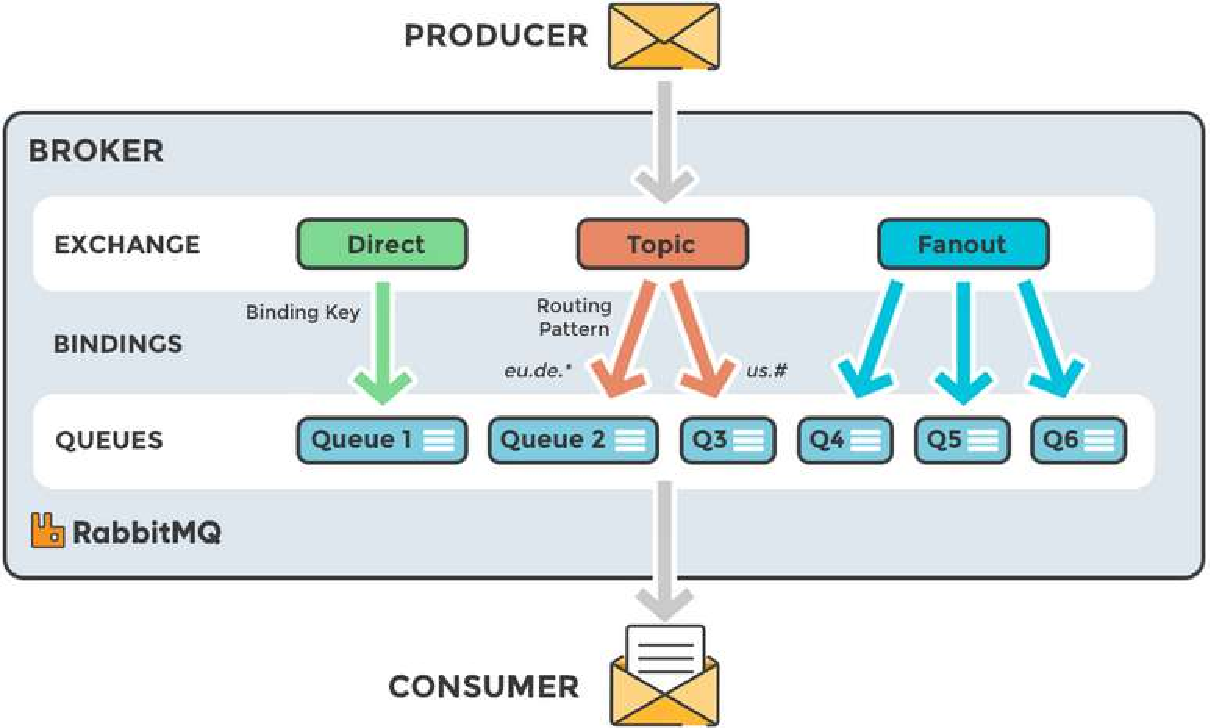
\includegraphics[width=12cm, height=6cm]{images/rabbitmq-componenti.pdf}
    \caption{Componenti del broker RabbitMQ. Fonte: RabbitMQ}
\end{figure}

Rispetto ad altri broker \Gls{rabbitmq} introduce l'\textit{queue} tra le sue componenti, e grazie a questa modifica implementa fedelmente il protocollo \acrshort{amqp}. Precedentemente vi erano solo i primi tre elementi sopracitati, con coda singola e metodo \acrshort{fifo}.\\
L'aspetto che contraddistingue \Gls{rabbitmq} rispetto ad altri broker (quali Kafka) è la capacità di lavorare molto velocemente quando le code sono quasi vuote: questo scenario è perfetto per la comunicazione tra microservizi. Inoltre la gestione delle code è più semplice, dato che il messaggio viene rimosso dalla coda una volta letto. Kafka invece è stato progettato per salvare i messaggi che arrivano per poterli leggere ed analizzare (tipicamente per il tracking degli utenti, logging) o per processarli in real-time.
%%%%%%%%%%  ALTRI SOFTWARE  %%%%%%%%%%
\section{Altri software utilizzati}\label{software}

Nell'implementazione di questo progetto sono state impiegati vari strumenti software:

\begin{itemize}
    \item \textbf{Visual Studio Code:} Visual Studio Code è un editor di codice sorgente leggero ma potente che viene eseguito sul desktop ed è disponibile per Windows, macOS e Linux. Viene fornito con il supporto integrato per JavaScript, TypeScript e Node.js e ha un ricco ecosistema di estensioni per altri linguaggi (come C++, Java, Python, PHP, Go) e runtime (come .NET e Unity) \cite{vscode}. Le estensioni utilizzate nel progetto sono state \textit{Extension Pack for Java}, \textit{Spring Boot Extension Pack}, \textit{Lombok Annotations Support for VS Code}, \textit{Docker}, \textit{Remote - Containers} e \textit{GitHub Pull Requests and Issues}.
    \item \textbf{Git:} Git è un sistema di controllo versione distribuito gratuito e open source progettato per gestire progetti sia piccoli che molto grandi con velocità ed efficienza \cite{git}. Nel progetto è stato adottato cosicché più programmatori potessero cooperare nella scrittura e nella risoluzione dei problemi.
    \item \textbf{Docker:} Docker è una piattaforma per lo sviluppo, la distribuzione e l'esecuzione di applicazioni. Consente di separare le applicazioni dall'infrastruttura in modo da poter distribuire rapidamente il software. Sfruttando le metodologie Docker si può ridurre significativamente il tempo intercorso tra la scrittura del codice e l'esecuzione in produzione \cite{docker}. Questo software è stato utilizzato per l'esecuzione di PostgreSQL e \Gls{rabbitmq} e per la creazione delle immagini dei microservizi.
    \item \textbf{Postman:}\label{postman} Postman è una piattaforma per la creazione e l'utilizzo di \Gls{api}. Postman semplifica ogni fase del ciclo di vita dell'\acrshort{api} e ottimizza la collaborazione in modo da poter creare \acrshort{api} migliori, più velocemente. La piattaforma include un set completo di strumenti che aiutano ad accelerare il ciclo di vita delle \acrshort{api}, dalla progettazione, test, documentazione e derisione alla condivisione e rilevabilità delle \acrshort{api} \cite{postman}.
    \item \textbf{DBeaver:} DBeaver è uno strumento di gestione del database universale per tutti coloro che hanno bisogno di lavorare con i dati in modo professionale. Con DBeaver si possono manipolare i dati, ad esempio in un normale foglio di calcolo, creare report analitici basati su record provenienti da diversi archivi di dati ed esportare le informazioni in un formato appropriato. Per gli utenti avanzati di database, DBeaver fornisce un potente editor SQL, numerose funzionalità di amministrazione, capacità di migrazione di dati e schemi, monitoraggio delle sessioni di connessione al database \cite{dbeaver}.
    \item \textbf{PostgreSQL:} \Gls{postgresql} è un \acrshort{dbms} ad oggetti. Il suo utilizzo nel progetto è frutto della necessità di rendere persistenti i dati, come utenti, password, lo storico delle sfide e log di sistema.
    \item \textbf{Angular:} Angular è una piattaforma per lo sviluppo di applicazioni web, basata su TypeScript. Come piattaforma, Angular include un framework basato su componenti per la creazione di applicazioni Web scalabili, una raccolta di librerie ben integrate che coprono un'ampia varietà di funzionalità, tra cui routing, gestione dei moduli, comunicazione client-server e una suite di strumenti per sviluppatori per aiutare a sviluppare, costruire, testare e aggiornare il codice.\cite{angular}
    \item \textbf{Maven}: Apache Maven è uno strumento di comprensione e gestione dei progetti software. Basato sul concetto di un modello a oggetti di progetto (\textit{POM}), Maven può gestire la creazione, il reporting e la documentazione di un progetto da un'informazione centrale \cite{maven}. Un \textit{POM} fornisce tutte le configurazioni di un singolo progetto, come per esempio il nome del progetto, la versione, il proprietario, dipendenze da altri progetti e le fasi di \textit{build} dell'applicazione.
\end{itemize}

Oltre agli strumenti sopraelencati nel progetto sono adottati anche diversi \gls{pattern}:
\begin{itemize}
    \item \textbf{Microservizi:} pattern opposto allo sviluppo monolitico in quanto ogni servizio deve poter essere sviluppato e distribuito in maniera indipendente. La comunicazione tra le varie componenti è solitamente basata su HTTP tramite chiamate REST.
    \item \textbf{Dependency injection:} Le due principali tecnologie impiegate nello sviluppo del prodotto, ovvero Angular e Spring, permettono entrambe di utilizzare il pattern \textit{dependecy injection} ovvero un \textit{design pattern} che permette di attuare l’\textit{inversion of control}. Le applicazioni Spring vengono istanziate all’interno di uno speciale container denominato \textit{IoC container} il quale si occupa di istanziare gli oggetti (\textit{beans}) dichiarati nel progetto e di reprire e iniettare tutte le dipendenze ad essi associate.
    \item \textbf{Lazy loading:} \textit{design pattern} utilizzato in \textit{Angular} che permette di caricare i moduli solo nel momento in cui effettivamente se ne ha bisogno ottenendo un guadagno in prestazioni di caricamento dell'applicazione.
\end{itemize}
\chapter{Progetto personale}

Dopo una prima fase puramente teorica il tirocinio è proseguito con un progetto personale per poter testare le conoscenze apprese. Quest'ultimo doveva includere il \textit{framework} Spring, il \textit{broker} RabbitMQ e permettere il salvataggio persistente dei dati su database PostgreSQL. Il progetto \cite{projtutorial} scelto aveva il compito di gestire le ordinazioni provenienti da più ristoranti. La struttura che lo compone è riportata di seguito:
\begin{flushleft}
\dirtree{%
.1 springbootrabbitmqexample.
.2 config.
.3 MessagingConfig.java.
.2 consumer.
.3 User.java.
.2 dto.
.3 Order.java.
.3 OrderRepository.java.
.3 OrderStatus.java.
.2 publisher.
.3 OrderPublisher.java.
.3 OrdersID.java.
.2 SpringbootRabbitmqExampleApplication.java.
} 
\end{flushleft}

\section{Gestione salvataggio ordini}
Per poter permettere il salvataggio persistente degli ordini ho utilizzato il \acrshort{dbms} PostgreSQL. Il database è composto da una singola tabella \texttt{orders} e gli ordini sono distinti univocamente dalla coppia (\texttt{orderId},\texttt{restaurant}).
\begin{table}[H]
    \centering
    \begin{tabular}{|p{3cm}|}
        \hline
        \textbf{orders}\\
        \hline
        \underline{orderId}\\
        \underline{restaurant}\\
        name\\
        qty\\
        price\\
        \hline
    \end{tabular}
    \caption{Tabella \texttt{orders}}
    \label{tab:orders}
\end{table}
La tabella \ref{tab:orders} viene generata dal codice contenuto nel file \texttt{Order}.
\begin{lstlisting}[language=Java, caption=Frammento codice tabella \texttt{orders}, basicstyle=\footnotesize]
@Entity
@Table(name = "orders")
@IdClass(OrdersID.class)
public class Order {
    @Id
    private String orderId;
    @Id
    private String restaurant;
    private String name;
    private int qty;
    private double price;
}
\end{lstlisting}
Nell'ordine, le annotazioni utilizzate servono per
\begin{enumerate}
    \item Indicare questa classe come modello per la generazione della tabella
    \item Specificare il nome della tabella
    \item Utilizzare una \textit{primary key} composta, creando anche una classe che racchiuda gli oggetti che compongono la \textit{primary key} stessa
\end{enumerate}
\begin{lstlisting}[language=Java, caption=Classe per utilizzare \textit{primary key} composta, basicstyle=\footnotesize]
public class OrdersID implements Serializable {
    private String orderId;
    private String restaurant;
}
\end{lstlisting}

\section{Gestione di invio e ricezione degli ordini}

Per poter permettere lo scambio di informazioni nell'applicazione ho configurato il broker di messaggi \textit{RabbitMQ} \ref{rabbitmq} nella classe \texttt{MessagingConfig} specificando i nomi di \textit{queue} ed \textit{exchange}.\\ L'invio degli ordini avviene mediante chiamate REST utilizzando Postman per l'invio della \textit{request} e la visualizzazione della \textit{response}. Una volta inviato l'ordine \texttt{OrderPublisher} ha il compito di ricevere queste chiamate ed estrarre le informazioni utili: nel body (in formato JSON) della chiamata vi è l'ordine mentre nel \textit{path} di quest'ultima vi è il nome del ristorante.
Esempio di chiamata REST:\\
\texttt{http://localhost:9292/order/lanterna}
\begin{lstlisting}[caption=Esempio contenuto del body,basicstyle=\footnotesize]
{
    "orderId": 1,
    "name": "spaghetti",
    "qty": 4,
    "price": 50
}
\end{lstlisting}
Dopo aver elaborato i dati ricevuti la classe \texttt{OrderPublisher} li invia al broker utilizzando l'oggetto \texttt{template} e successivamente li salva in modo persistente richiamando il metodo \texttt{save} dell'oggetto \texttt{orderRepo}:
\begin{lstlisting}[language=Java, caption=Frammento del codice della classe \texttt{OrderPublisher} e relativo metodo \texttt{bookOrder}, basicstyle=\footnotesize]
@Autowired
private RabbitTemplate template;
@Autowired
private OrderRepository orderRepo;
...
template.convertAndSend(MessagingConfig.EXCHANGE,
    MessagingConfig.ROUTING_KEY, orderStatus);
orderRepo.save(order);
...
\end{lstlisting}
Per finire nel progetto è stato inserito anche una classe \texttt{User} il cui compito è quello di ricevere i messaggi dal broker, leggerli e stampare a schermo i dettagli dell'ordinazione appena effettuata.
\begin{lstlisting}[language=Java, caption=Frammento del codice della classe \texttt{User}, basicstyle=\footnotesize]
@RabbitListener(queues = MessagingConfig.QUEUE)
public void consumeMessageFromQueue(OrderStatus orderStatus) {
    System.out.println("Message recieved: " + orderStatus +
    "\nOrder details: " + orderStatus.getOrder().toString());
}
\end{lstlisting}
\chapter{Challenginator}\label{challenginator}

L'analisi che segue è stata svolta da persone terze quando il progetto è stato avviato \cite{canovese}.\\
\textit{Challenginator} è una \textit{web application} che permette l'invio, la ricezione ed il tracciamento di sfide tra i membri di un team. Mediante la \textit{user interface} ogni utente può effettuare la registrazione e, dopo il processo di autenticazione tramite login, l'accesso alla propria area personale.
Da quest'ultima l'utente ha accesso a:
\begin{itemize}
    \item Home: pagina riepilogativa
    \item Dashboard: pagina con accesso rapido alle sfide passate, alla procedura di lancio di una nuova sfida ed elencazione di sfide in cui si è stati sfidati, si sfida o si fa da valutatore
    \item Preferenze di notifica: pagina dove l'utente decide quali tipologie di notifica ricevere
    \item Storico: pagina contenente lo storico delle sfide
    \item Nuova Challenge: pagina dove è possibile lanciare una nuova sfida
    \item Logout
\end{itemize}
Ogni utente può sfidare un collega attraverso l'apposito form di inserimento di una nuova sfida ed in modo automatico verrà assegnato un valutatore. Quest'ultimo è il soggetto, gerarchicamente a livello superiore, che decreterà la riuscita od il fallimento della sfida una volta completata da parte dello sfidato.

%%%%%%%%%%  ANALISI REQUISITI   %%%%%%%%%%
\section{Analisi dei requisiti}

Lo scopo del prodotto è stato riportato nella sezione precedente.
Durante l'intero flusso dell'applicazione gli attori del sistema sono:
\begin{itemize}
    \item \textbf{Utente non autenticato:} identifica un utente che non ha ancora effettuato l'accesso al rispettivo account
    \item \textbf{Utente autenticato:} identifica un utente che ha effettuato correttamente il login e può essere identificato a sua volta come:
    \begin{itemize}
        \item \textbf{Sfidante:} utente che ha inserito una sfida contro un utente terzo
        \item \textbf{Sfidato:} utente che ha ricevuto una sfida da un utente terzo
        \item \textbf{Valutatore:} utente che deve decretare la riuscita o meno di una sfida
    \end{itemize}
\end{itemize}

%%%%%%%%%%  CASI D'USO  %%%%%%%%%%
\subsection{Casi d'uso}

I casi d'uso individuati sono elencati di seguito.

\begin{table}[H]
    \centering
    \begin{tabular}{|p{3cm}p{11.15cm}|}
        \hline
        %\multicolumn{2}{|c|}{\textbf{UC-1: Login utente}} \\\hline
        \textbf{Attore primario} & utente non autenticato \\
        \textbf{Descrizione} & autenticazione utente \\
        \textbf{Precondizioni} & l’utente non si è ancora autenticato nell’applicazione \\
        \textbf{Input} & l’utente inserisce ed invia i dati per il login \\
        \textbf{Postcondizioni} & il cliente è autenticato \\\hline
    \end{tabular}
    \caption{UC-1: Login utente}
\end{table}
\begin{table}[H]
    \centering
    \begin{tabular}{|p{3cm}p{11.15cm}|}
        \hline
        %\multicolumn{2}{|c|}{\textbf{UC-1: Login utente}} \\\hline
        \textbf{Attore primario} & utente non autenticato \\
        \textbf{Descrizione} & registrazione nuovo utente \\
        \textbf{Precondizioni} & l’utente non si è ancora autenticato nell’applicazione \\
        \textbf{Input} & l’utente inserisce ed invia i dati per la creazione del proprio account \\
        \textbf{Postcondizioni} & il cliente è autenticato \\\hline
    \end{tabular}
    \caption{UC-2: Registrazione utente}
\end{table}
\begin{table}[H]
    \centering
    \begin{tabular}{|p{3cm}p{11.15cm}|}
        \hline
        %\multicolumn{2}{|c|}{\textbf{UC-1: Login utente}} \\\hline
        \textbf{Attore primario} & utente autenticato (sfidante, sfidato, valutatore) \\
        \textbf{Descrizione} & l’utente vuole visualizzare le sfide in cui è coinvolto come sfidato, sfidante o valutatore \\
        \textbf{Precondizioni} & l’utente ha effettuato il login \\
        \textbf{Input} & l’utente clicca sulla voce di menù dashboard, se non la sta già visualizzando a seguito del login \\
        \textbf{Postcondizioni} & l’utente visualizza la \textit{dashboard} contenente tutte le sfide in cui è coinvolto a vario titolo \\\hline
    \end{tabular}
    \caption{UC-3: Visualizzazione lista sfide (\textit{dashboard})}
\end{table}
\begin{table}[H]
    \centering
    \begin{tabular}{|p{3cm}p{11.15cm}|}
        \hline
        %\multicolumn{2}{|c|}{\textbf{UC-1: Login utente}} \\\hline
        \textbf{Attore primario} & utente autenticato - sfidante \\
        \textbf{Descrizione} & l’utente che ha lanciato la sfida vuole cancellarla \\
        \textbf{Precondizioni} & l’utente sta visualizzando la dashboard riepilogativa ed è l’utente sfidante \\
        \textbf{Input} & l’utente clicca sul pulsante per cancellare la sfida \\
        \textbf{Postcondizioni} & l’utente ha cancellato la sfida \\\hline
    \end{tabular}
    \caption{UC-3.1: Cancellazione challenge}
\end{table}
\begin{table}[H]
    \centering
    \begin{tabular}{|p{3cm}p{11.15cm}|}
        \hline
        %\multicolumn{2}{|c|}{\textbf{UC-1: Login utente}} \\\hline
        \textbf{Attore primario} & utente autenticato - sfidato \\
        \textbf{Descrizione} & l’utente vuole accettare una sfida che gli viene proposta \\
        \textbf{Precondizioni} & l’utente sta visualizzando la \textit{dashboard} riepilogativa, e una sfida in cui è identificato come sfidato è in attesa \\
        \textbf{Input} & l’utente clicca sul pulsante per accettare la sfida \\
        \textbf{Postcondizioni} & l’utente ha accettato la sfida \\\hline
    \end{tabular}
    \caption{UC-3.2: Accettazione challenge}
\end{table}
\begin{table}[H]
    \centering
    \begin{tabular}{|p{3cm}p{11.15cm}|}
        \hline
        %\multicolumn{2}{|c|}{\textbf{UC-1: Login utente}} \\\hline
        \textbf{Attore primario} & utente autenticato - sfidato \\
        \textbf{Descrizione} & l’utente vuole rifiutare una sfida che gli viene proposta \\
        \textbf{Precondizioni} & l’utente sta visualizzando la \textit{dashboard} riepilogativa, e una sfida in cui è identificato come sfidato è in attesa \\
        \textbf{Input} & l’utente clicca sul pulsante per rifiutare la sfida \\
        \textbf{Postcondizioni} & l’utente ha rifiutato la sfida \\\hline
    \end{tabular}
    \caption{UC-3.3: Rifiuto challenge}
\end{table}
\begin{table}[H]
    \centering
    \begin{tabular}{|p{3cm}p{11.15cm}|}
        \hline
        %\multicolumn{2}{|c|}{\textbf{UC-1: Login utente}} \\\hline
        \textbf{Attore primario} & utente autenticato - sfidato \\
        \textbf{Descrizione} & l’utente vuole dichiarare la sfida in cui è sfidato come completata \\
        \textbf{Precondizioni} & l’utente sta visualizzando la \textit{dashboard} riepilogativa, e vuole dichirare la sfida (in cui risulta sfidato) come completata \\
        \textbf{Input} & l’utente clicca sul pulsante per completare la sfida \\
        \textbf{Postcondizioni} & l’utente ha modificato lo stato della sfida \\\hline
    \end{tabular}
    \caption{UC-3.4: Dichiarare la sfida come completata}
\end{table}
\begin{table}[H]
    \centering
    \begin{tabular}{|p{3cm}p{11.15cm}|}
        \hline
        %\multicolumn{2}{|c|}{\textbf{UC-1: Login utente}} \\\hline
        \textbf{Attore primario} & utente autenticato - sfidato \\
        \textbf{Descrizione} & l’utente vuole arrendersi in una sfida \\
        \textbf{Precondizioni} & l’utente sta visualizzando la \textit{dashboard} riepilogativa, e vuole arrendersi in una sfida \\
        \textbf{Input} & l’utente clicca sul pulsante per arrendersi \\
        \textbf{Postcondizioni} & l’utente ha modificato lo stato della sfida \\\hline
    \end{tabular}
    \caption{UC-3.5: Arrendersi in una sfida}
\end{table}
\begin{table}[H]
    \centering
    \begin{tabular}{|p{3cm}p{11.15cm}|}
        \hline
        %\multicolumn{2}{|c|}{\textbf{UC-1: Login utente}} \\\hline
        \textbf{Attore primario} & utente autenticato \\
        \textbf{Descrizione} & l’utente vuole visualizzare il dettaglio di una sfida \\
        \textbf{Precondizioni} & l’utente sta visualizzando la \textit{dashboard} riepilogativa \\
        \textbf{Input} & l’utente clicca sul pulsante per visualizzare i dettagli della sfida, quali inizio e fine, tempo rimanente, la descrizione completa... \\
        \textbf{Postcondizioni} & l’utente visualizza la pagina di dettaglio della sfida \\\hline
    \end{tabular}
    \caption{UC-4: Visualizzazione dettaglio sfida}
\end{table}
\begin{table}[H]
    \centering
    \begin{tabular}{|p{3cm}p{11.15cm}|}
        \hline
        %\multicolumn{2}{|c|}{\textbf{UC-1: Login utente}} \\\hline
        \textbf{Attore primario} & utente autenticato \\
        \textbf{Descrizione} & l’utente vuole inserire una nuova sfida \\
        \textbf{Precondizioni} & l’utente clicca il pulsante di creazione nuova sfida \\
        \textbf{Input} & l’utente inserisce i dati richiesti per lanciare una sfida \\
        \textbf{Postcondizioni} & l’utente ha lanciato una sfida \\\hline
    \end{tabular}
    \caption{UC-5: Inserimento nuova sfida}
\end{table}
\begin{table}[H]
    \centering
    \begin{tabular}{|p{3cm}p{11.15cm}|}
        \hline
        %\multicolumn{2}{|c|}{\textbf{UC-1: Login utente}} \\\hline
        \textbf{Attore primario} & utente autenticato \\
        \textbf{Descrizione} & l’utente vuole visualizzare il dettaglio di una sfida \\
        \textbf{Precondizioni} & l’utente sta visualizzando la \textit{dashboard} riepilogativa \\
        \textbf{Input} & l’utente clicca il pulsante per visualizzare il dettaglio della sfida \\
        \textbf{Postcondizioni} & l’utente visualizza la pagina di dettaglio della sfida \\\hline
    \end{tabular}
    \caption{UC-6: Visualizzazione storico sfide}
\end{table}
\begin{table}[H]
    \centering
    \begin{tabular}{|p{3cm}p{11.15cm}|}
        \hline
        %\multicolumn{2}{|c|}{\textbf{UC-1: Login utente}} \\\hline
        \textbf{Attore primario} & utente autenticato \\
        \textbf{Descrizione} & l’utente vuole decidere quali notifiche ricevere \\
        \textbf{Precondizioni} & l’utente seleziona le \textit{checkbox} \\
        \textbf{Input} & l’utente clicca il pulsante di selezione preferenze di notifica, come in figura \ref{fig:prefnot} \\
        \textbf{Postcondizioni} & l’utente salva le sue preferenze di notifica \\\hline
    \end{tabular}
    \caption{UC-7: Scelta preferenze di notifica}
\end{table}

%%%%%%%%%% TRACCIAMENTO REQUISITI   %%%%%%%%%%
\subsection{Tracciamento dei requisiti}
Per elencare i requisiti individuati correlati ai casi d'uso utilizzo la seguente codifica:
\begin{center}
    \texttt{R[Importanza][Tipologia]-[Codice]}
\end{center}
\begin{itemize}
    \item \textbf{Importanza:} indica l'importanza di tale requisito attraverso i valori
    \begin{itemize}
        \item \textbf{1} requisito obbligatorio
        \item \textbf{2} requisito desiderabile
        \item \textbf{3} requisito opzionale
    \end{itemize}
    \item \textbf{Tipologia}
    \begin{itemize}
        \item \textbf{V} requisito di vincolo
        \item \textbf{F} requisito funzionale
        \item \textbf{Q} requisito di qualità
    \end{itemize}
    \item \textbf{Codice:} identificatore univoco in forma gerarchica padre/figlio
\end{itemize}
\begin{center}
    \textbf{[CodiceBase](.[CodiceSottoCaso])*}
\end{center}
Il CodiceBase identifica il caso d'uso generico. Il CodiceSottoCaso (opzionale) identifica i sottocasi.

\begin{longtable}[H]{ll}
    \caption{Tabella tracciamento dei requisiti funzionali} \\
    \textbf{Requisito} & \textbf{Descrizione} \\\hline
    R1F-1 & L’utente deve poter fare il login per accedere al sito \\\hline
    R1F-1.2 & Il sistema deve fare il display dell’errore di autenticazione \\\hline
    R1F-2 & L’utente non autenticato deve potersi registrare \\\hline
    R1F-2.1 & Il sistema deve fare il display dell’errore di registrazione \\\hline
    R1F-3 & L’utente deve poter visualizzare la dashboard \\\hline
    R1F-3.1 & L’utente deve poter visualizzare le sfide in cui è coinvolto come sfidato \\\hline
    R1F-3.1 & L’utente deve poter visualizzare le sfide in cui è coinvolto come sfidante \\\hline
    R1F-3.1 & L’utente deve poter visualizzare le sfide in cui è coinvolto come valutatore \\\hline
    R1F-3.2 & L’utente deve poter accettare una sfida che gli viene proposta \\\hline
    R1F-3.3 & L’utente deve poter cancellare una sfida lanciata \\\hline
    R1F-3.4 & L’utente deve poter segnare come completata una sfida \\\hline
    R1F-3.5 & L’utente deve poter arrendersi in una sfida \\\hline
    R1F-3.6 & L’utente valutatore deve poter valutare con succeso una sfida \\\hline
    R1F-3.7 & L’utente valutatore deve poter valutare il fallimento di una sfida \\\hline
    R1F-4 & L’utente deve poter inserire una nuova sfida \\\hline
    R1F-4.1 & L’utente deve poter selezionare chi sfidare \\\hline
    R1F-4.2 & L’utente deve poter specificare il titolo della sfida \\\hline
    R1F-4.3 & L’utente deve poter specificare il dettaglio della sfida \\\hline
    R1F-4.4 & L’utente deve poter inserire il termine per completare la sfida \\\hline
    R1F-5 & L’utente deve poter visualizzare lo storico delle sfide \\\hline
    R1F-6 & L’utente deve poter visualizzare il dettaglio di una sfida \\\hline
    R1F-6.1 & L’utente deve poter visualizzare il dettaglio cronologico della sfida \\\hline
    R1F-7 & L'utente deve poter decidere quali notifiche ricevere \\\hline
\end{longtable}

\begin{longtable}[H]{ll}
    \caption{Tabella del tracciamento dei requisiti di vincolo} \\
    \textbf{Requisito} & \textbf{Descrizione} \\\hline
    R1V-1 & Il backend deve essere realizzato tramite il framework Spring \\\hline
    R1V-2 & Il frontend deve essere realizzato tramite il framework Angular \\\hline
    R1V-3 & Il backend deve adottare un’architettura a microservizi \\\hline
    R1V-3 & La persistenza dei dati deve essere garantita con un database PostgreSQL \\\hline
    R1V-4 & La GUI deve essere realizzata mediante l’utilizzo della libreria \textit{Bootstrap} \\\hline
\end{longtable}

%%%%%%%%%%  PROBLEMATICHE   %%%%%%%%%%
\subsection{Problematiche riscontrate}
Dall'analisi preventiva dei rischi sono state individuate alcune possibili problematiche a cui si potrà andare incontro:
\begin{enumerate}
    \item \textbf{Conoscenza delle tecnologie}
    \begin{itemize}
        \item \textbf{Descrizione:} possibile rallentamento nell'attività di sviluppo a causa dell'utilizzo delle nuove tecnologie acquisite nella fasi di studio individuale \ref{teoria}
        \item \textbf{Soluzione:} autoverifica periodica delle conoscenze acquisite, testandole con piccoli progetti
    \end{itemize}
    \item \textbf{Inclusione di nuovi requisiti}
    \begin{itemize}
        \item \textbf{Descrizione:} l'utilizzo di un metodo di sviluppo \textit{agile} potrebbe complicare l'aggiunta di nuovi requisiti da soddisfare in corso d'opera
        \item \textbf{Soluzione:} coinvolgere il committente, in questo caso il tutor, in una ciclica analisi dei requisiti, così da intervenire solamente per piccoli aggiustamenti
    \end{itemize}
\end{enumerate}

%%%%%%%%%%  PROGETTAZIONE   %%%%%%%%%%
\section{Progettazione}

L'architettura della componente \textit{backend} del progetto \textit{Challenginator} è realizzata con i microservizi, ovvero servizi di piccole dimensioni che per poter comunicare tra loro utilizzano API ben definite.
La comunicazione con il lato \textit{frontend} avviene utilizzando chiamate all'API Gateway, microservizio che si interpone tra \textit{frontend} e \textit{backend}.
La comunicazione tra microservizi avviene mediante il broker \gls{rabbitmq}.\\
Il progetto è composto dai seguenti microservizi:
\begin{itemize}
    \item api-gateway
    \item challenge-service
    \item eurekaserver
    \item logger-service
    \item notification-service
    \item scheduler-service
    \item user-service
\end{itemize}
Il database che permette il salvataggio permanente dei dati è composto dalle seguenti tabelle:\\
Tabella \texttt{app\_user} per salvare i dati riguardanti gli utenti. Le password prima di esser salvate saranno crittografate.
\begin{table}[H]
    \centering
    \begin{tabular}{|p{4cm}|}
    \hline
    \textbf{app\_user}\\\hline
    \underline{id}\\
    app\_user\_role\\
    boss\_id\\
    email\\
    enabled\\
    locked\\
    name\\
    password\\
    score\\
    surname\\\hline
    \end{tabular}
    \caption{Tabella \texttt{app\_user} del database \texttt{challenginator}}
\end{table}

Tabella \texttt{log} per salvare i log dei vari microservizi.
\begin{table}[H]
    \centering
    \begin{tabular}{|p{4cm}|}
    \hline
    \textbf{log}\\\hline
    \underline{id}\\
    level\\
    log\_message\\
    service\_name\\
    time\\\hline
    \end{tabular}
    \caption{Tabella \texttt{log} del database \texttt{challenginator}}
\end{table}

Tabella \texttt{challenge} per salvare i dettagli delle singole sfide.
\begin{table}[H]
    \centering
    \begin{tabular}{|p{4cm}|}
    \hline
    \textbf{challenge}\\\hline
    \underline{id}\\
    challenged\\
    challenger\\
    deadline\\
    description\\
    evaluator\\
    result\\
    status\\
    timestamp\_acceptance\\
    timestamp\_creation\\
    title\\\hline
    \end{tabular}
    \caption{Tabella \texttt{challenge} del database \texttt{challenginator}}
\end{table}

Tabella \texttt{user\_preference} per salvare le preferenze di notifica di ogni utente. I campi di questa tabella (escluso \texttt{id}) sono di tipo \texttt{boolean}.
\begin{table}[H]
    \centering
    \begin{tabular}{|p{4cm}|}
    \hline
    \textbf{user\_preference}\\\hline
    \underline{userid}\\
    challenge\_accepted\\
    challenge\_completed\\
    challenge\_created\\
    challenge\_deleted\\
    challenge\_giveup\\
    challenge\_refused\\
    challenge\_terminated\\
    challenge\_updated\\\hline
    \end{tabular}
    \caption{Tabella \texttt{user\_preference} del database \texttt{challenginator}}
\end{table}
\chapter{Servizio di notifica}\label{service}

Il servizio di notifica implementato nell'applicazione utilizza RabbitMQ per raccogliere le informazione da trasmettere, genera il messaggio e poi lo spedisce mediante e-mail.\\
La struttura del microservizio è riportata di seguito:
\begin{flushleft}
\dirtree{%
.1 notificationservice.
.2 challenge.
.3 Challenge.java.
.3 ChallengeEventType.java.
.3 ChallengeResult.java.
.3 ChallengeStatus.java.
.2 mail.
.3 EmailService.java.
.3 EmailServiceConfig.java.
.3 SimpleMailMessageBuilder.java.
.2 messaging.
.3 Receiver.java.
.2 user.
.3 AppUser.java.
.3 UserPreference.java.
.3 UserPreferenceRepository.java.
.3 UserPreferenceService.java.
.2 AppConfig.java.
.2 Controller.java.
.2 NotificationServiceApplication.java.
}
\end{flushleft}

%%%%%%%%%%  PREFERENZE NOTIFICHE    %%%%%%%%%%
\section{Preferenze notifiche}

Nella web app vi è un'apposita sezione per le preferenze di notifica per avere un controllo granulare su quest'ultime. Come si può notare dalla figura \ref{fig:prefnot} vi sono vari campi dotati di check-box per poter selezionare quali notifiche ricevere.

\begin{figure}[H]
    \centering
    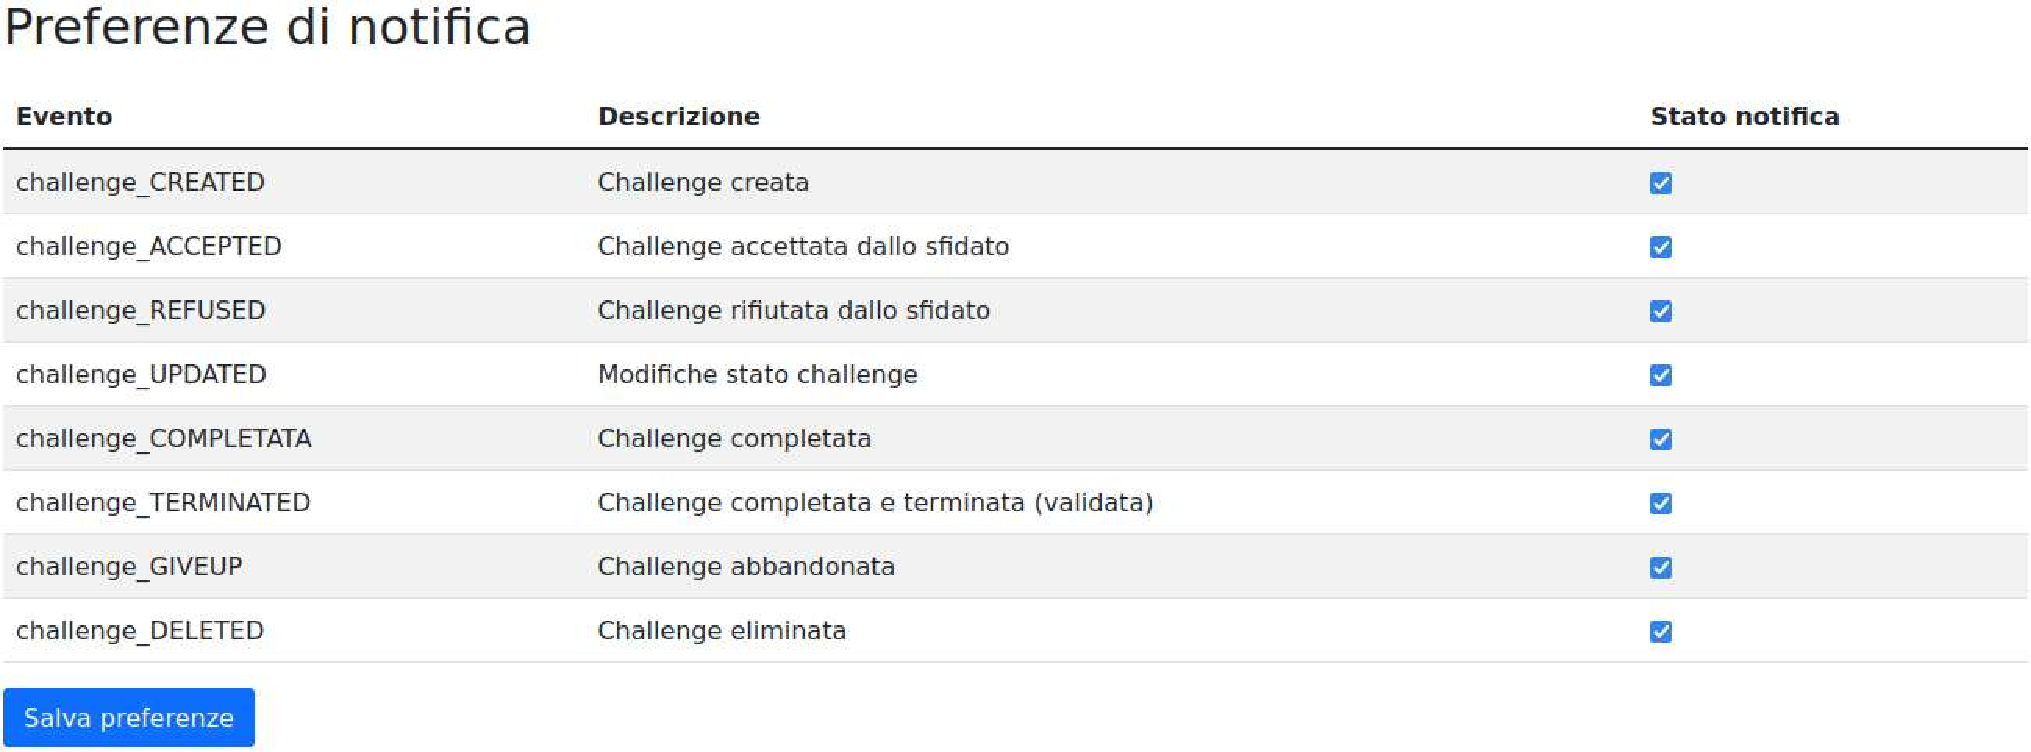
\includegraphics[width=1\textwidth]{images/preferenze-notifica.pdf}
    \caption{Preferenze di notifica webapp}
    \label{fig:prefnot}
\end{figure}

Al primo accesso si spuntano i check-box interessati e si salvano le proprie preferenze. Nel salvataggio viene creata una nuova istanza nella tabella \texttt{user\_preference}, contenente i campi scelti dall'utente, così da salvare il tutto permanentemente.

\begin{lstlisting}[language=Java, caption=Frammento codice preferenze utente, basicstyle=\footnotesize]
@Entity
public class UserPreference {
    @Id
    private Long userID;
    private boolean CHALLENGE_CREATED;
    private boolean CHALLENGE_ACCEPTED;
    private boolean CHALLENGE_REFUSED;
    private boolean CHALLENGE_COMPLETED;
    private boolean CHALLENGE_UPDATED;
    private boolean CHALLENGE_DELETED;
    private boolean CHALLENGE_GIVEUP;
    private boolean CHALLENGE_TERMINATED;
}
\end{lstlisting}

Come si può notare dal precedente frammento di codice, le istanze nel database hanno come \textit{primary key} l'id utente, mentre i rimanenti campi sono \texttt{boolean} dato che il dato contenuto è la preferenza dei check-box.\\
Dopo l'operazione di aggiornamento delle preferenze, durante il flusso dell'applicazione (utenti si sfidano, utenti completano le sfide, ..), verranno inviate ai rispettivi utenti le notifiche richieste: il mittente è \texttt{rabbitmailtest@gmail.com}, indirizzo creato appositamente per questa parte del progetto, l'oggetto sarà l'evento che ha scatenato l'invio dell'email ed il corpo del messaggio conterrà le informazioni specifiche, quali sfidato, sfidante, giudice, tempo di completamento, titolo e descrizione della sfida.

\begin{figure}[H]
    \centering
    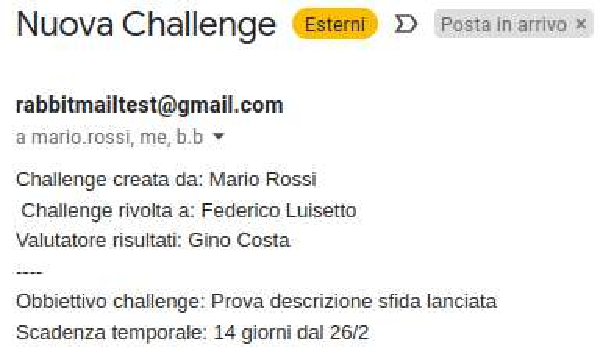
\includegraphics[width=9cm, height=5cm]{images/prova-email.pdf}
    \caption{Esempio mail}
\end{figure}

%%%%%%%%%%  GENERAZIONE MAIL   %%%%%%%%%%
\section{Generazione e-mail}

La generazione e l'invio delle e-mail sono gestiti dalla classe \texttt{EmailService}, appartenente alla sezione \textit{mail} del servizio. Quest'ultima delega la configurazione del servizio mail (protocollo, porta, nome utente, password, ...) a \texttt{EmailServiceConfig} e la costruzione della mail stessa (mittente, ricevitore, oggetto e corpo) a \texttt{SimpleMailMessageBuilder}
\begin{lstlisting}[language=Java, caption=Generazione corpo email, basicstyle=\footnotesize]
public void process(Challenge challenge, ChallengeEventType eventType)
{
    try {
        AppUser challenger = getUser(challenge.getChallenger());
        AppUser challenged = getUser(challenge.getChallenged());
        AppUser evaluator = getUser(challenge.getEvaluator());
        
        SimpleMailMessageBuilder mailBuilder = 
            new SimpleMailMessageBuilder(
            challenge,
            eventType,
            emailServiceConfig.username,
            challenger,
            challenged,
            evaluator);
        SimpleMailMessage message = mailBuilder.build();
        emailSender.send(message);
    } catch (Exception e) {
        e.printStackTrace();
    }
}
\end{lstlisting}

L'intero meccanismo di invio è messo in moto dalla classe \texttt{Receiver}, appartenente alla sezione \textit{messaging}, che mediante RabbitMQ si mette in ascolto dei nuovi messaggi nella coda \texttt{challengeQueue}. All'arrivo di un nuovo messaggio nella coda viene richiamato il metodo della classe \texttt{EmailService} sopra riportato.

\begin{lstlisting}[language=Java, caption=Ricezione update ed invio notifica, basicstyle=\footnotesize]
@EnableRabbit
@Service
public class Receiver {
    @Autowired
    EmailService emailService;
    static final public String queueName = "challengeQueue";
    @RabbitListener(queues = queueName)
    public void receiveMessage(byte[] newChallenge, 
        @Header(name="event_type") String eventType) {
    ObjectMapper mapper = new ObjectMapper();
    Challenge challenge = null;
    try {
      challenge = mapper.readValue(new String(newChallenge), 
        Challenge.class);
    } catch(JsonProcessingException e) {
      e.printStackTrace();
    }
    emailService.process(challenge, 
        ChallengeEventType.valueOf(eventType));
  }
}
\end{lstlisting}
\chapter{Logger}\label{logger}

%%%%%%%%%%  LOG4J   %%%%%%%%%%
\section{Log4j}

In prima analisi per il progetto si era pensato di utilizzare \textit{Log4j}, dato il larghissimo impiego, per il logging degli eventi da salvare poi su un file. Per poterlo utilizzare all'interno di Challenginator si sono aggiungente le dovute dipendenze, mediante \textit{Maven}, e un file \texttt{log4j2-spring.xml} dove venivano specificate le impostazioni del logger per ogni microservizio coinvolto.\\
Nel contempo però è emersa una vulnerabilità che ha scosso l'intero mondo informatico: si è scoperta la falla \textit{Log4Shell} (\texttt{CVE-2021-44228}) che permetteva ad un utente malintenzionato di controllare i messaggi di registro o i parametri dei messaggi di registro. In questa maniera era possibile eseguire codice arbitrario caricato dai server LDAP quando è abilitata la sostituzione della ricerca dei messaggi.
\begin{figure}[H]
    \centering
    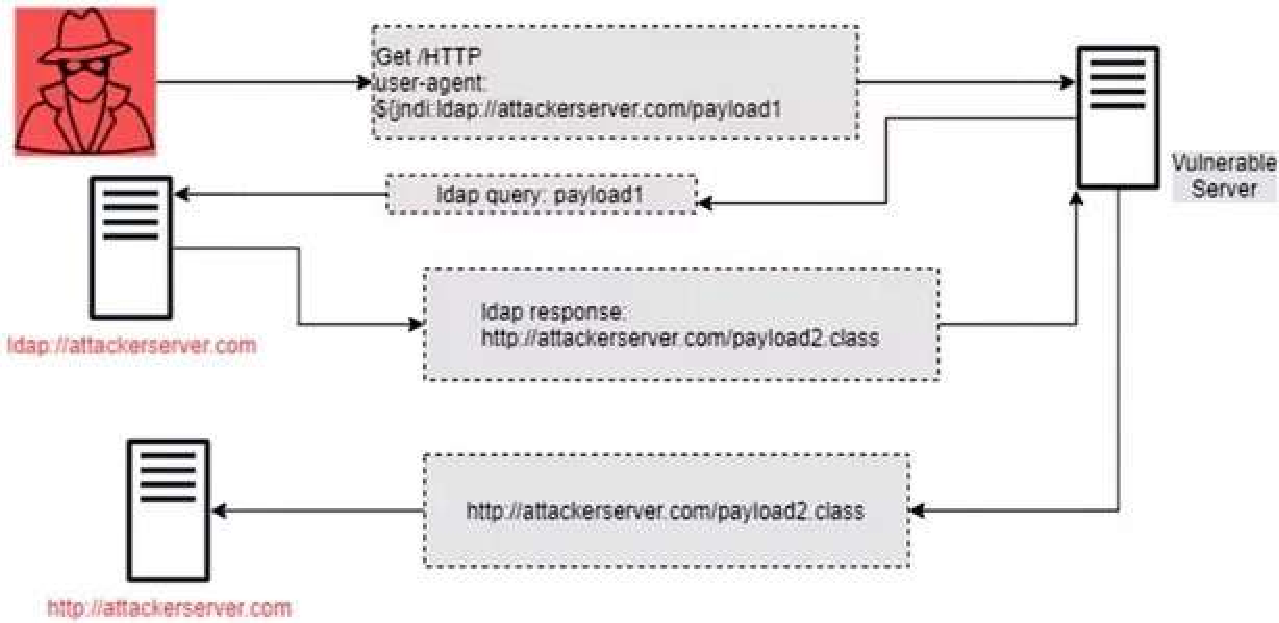
\includegraphics[width=9cm, height=4cm]{images/log4j-log4shell-bug.pdf}
    \caption{Funzionamento attacco mediante Log4Shell. Fonte: LFFL}
\end{figure}

Il CISA ha fornito una chiara rappresentazione, mediante uno schema chart, del grado di vulnerabilità del proprio sistema se si utilizza \textit{Log4j}. \cite{log4j}

\begin{figure}[H]
    \centering
    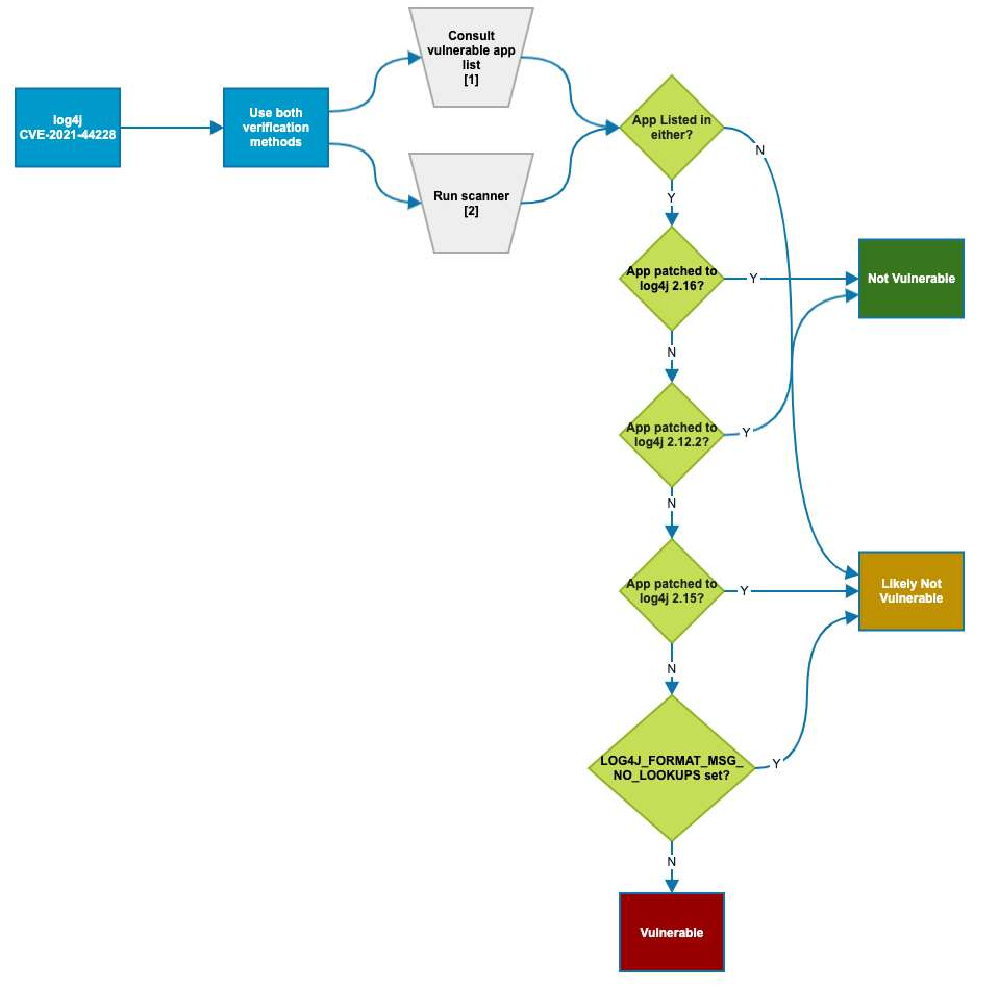
\includegraphics[width=1\textwidth]{images/log4j-bug.pdf}
    \caption{Grafico sulla vulnerabilità di prodotti che utilizzano Log4j. Fonte: CISA}
\end{figure}

Dopo questa vulnerabilità abbiamo deciso di affidarci ad un altro progetto per il logging: Logback.

%%%%%%%%%%  LOGBACK   %%%%%%%%%%
\section{Logback}

Logback \cite{logback} è uno dei più utilizzati framework per il logging nella community Java dato che, rispetto a Log4j, offre una più veloce implementazione, più opzioni di configurazione e maggiore flessibilità  nell'archiviazione di vecchi file.\\
Per inserire questo sistema di log all'interno del progetto è necessario inserire le relative dipendenze maven nel file \texttt{pom.xml}:
\begin{lstlisting}[language=XML, caption=Dipendenze Maven Logback, basicstyle=\footnotesize]
<dependency>
    <groupId>ch.qos.logback</groupId>
    <artifactId>logback-core</artifactId>
    <version>1.2.10</version>
</dependency>
<dependency>
    <groupId>ch.qos.logback</groupId>
    <artifactId>logback-classic</artifactId>
    <version>1.2.10</version>
</dependency>
<dependency>
    <groupId>org.slf4j</groupId>
    <artifactId>slf4j-api</artifactId>
    <version>1.7.32</version>
</dependency>
\end{lstlisting}

Per la configurazione è necessario creare un file di nome \texttt{logback-spring.xml} ed inserirlo nel progetto. In questo file si possono configurare gli \textit{appender}, all'interno dei quali Logback scriverà i messaggi di log; nel progetto inizialmente i log erano riportati nel terminale dell'applicazione e salvati in un file, successivamente con l'adozione di Docker venivano inviati direttamente ad una tabella del database.\\
Per poter registrare gli eventi bisogna, all'interno delle singole classi, dichiarare una variabile \texttt{Logger} ed inviare i singoli messaggi.
\begin{lstlisting}[language=Java, caption=Esempio Logger Logback, basicstyle=\footnotesize]
public class Example {
    private static final Logger logger 
      = LoggerFactory.getLogger(Example.class);

    public static void main(String[] args) {
        logger.info("Example log {}",Example.class.getSimpleName());
    }
}
\end{lstlisting}
\cite{logbackguide}.
Le funzioni da chiamare dipendono dal livello di importanza dell'informazione da trasmettere:
\begin{itemize}
    \item \texttt{.error} per il livello ERROR. Indica un errore di esecuzione o una condizione improvvisa.
    \item \texttt{.warn} per il livello WARN. Indica una condizione inaspettata o anomala di esecuzione, che però non necessariamente ha comportato un errore.
    \item \texttt{.info} per il livello INFO. Usato per segnalare gli eventi di esecuzione.
    \item \texttt{.debug} per il livello DEBUG. Usato nella fase di debug dell'applicazione.
\end{itemize}
Questa soluzione sembrava quella ottimale, ma sfortunatamente la comunicazione tra l'applicazione e il database non si instaurava e abbiamo dovuto intraprendere una nuova strada, una soluzione custom per il logging.

%%%%%%%%%%  CUSTOM LOG   %%%%%%%%%%
\section{Logger Custom}

La configurazione personalizzata è composta da  un nuovo servizio denominato \textit{logger\textunderscore service} che raccoglie tutti i messaggi di log dai vari microservizi e li invia al database ed una nuova componente in ogni microservizio atta all'invio dei messaggi di log al servizio dedicato.\\
La struttura del microservizio è riportata di seguito:
\begin{flushleft}
\dirtree{%
.1 logger\_service.
.2 controller.
.3 Controller.java.
.2 log.
.3 Log.java.
.3 LogLevel.java.
.3 LogRepository.java.
.2 messaging.
.3 LogReceiver.java.
.3 MessagingConfig.java.
.2 LogService.java.
.2 LoggerServiceApplication.java.
}
\end{flushleft}

%%%%%%%%%%  LOGGER SERVICE  %%%%%%%%%%
\subsection{Logger service}

Questo nuovo servizio è composto da principalmente tre parti:
\begin{itemize}
    \item \textit{controller}: riceve delle \textit{request} tramite URL e genera le \textit{response} corrispondenti
    \item \textit{log}: genera la classe \texttt{Log}, crea la relativa tabella nel database e si occupa delle \acrlong{jpa}
    \item \textit{messaging}: configura RabbitMQ per questo servizio, riceve le informazioni sui log dai vari microservizi e richiede il salvataggio persistente di questi ultimi 
\end{itemize}

Per la creazione del \textit{controller} si utilizzano le potenzialità del framework Spring. Mediante l'annotazione \texttt{RestController} (include le annotazioni \texttt{Controller} e \texttt{ResponseBody}) si ottiene un \textit{controller} specializzato, capace di gestire le \textit{request} mediante metodi in grado di trasformare automaticamente gli oggetti ritornati in \textit{HttpResponse}. L'annotazione \texttt{GetMapping} gestisce le chiamate GET al link specificato; tali percorsi sono esposti alla porta 8080 mediante l'\textit{API gateway}.

\begin{lstlisting}[language=Java, caption=Controller logger service, basicstyle=\footnotesize]
@RestController
public class Controller {
    @Autowired
    LogService logService;
    // restituisce tutti i log
    @GetMapping("/logs/getalllogs")
    public List<Log> getController() {
        return logService.getAll();
    }
    // controller di prova, aggiunge log fasullo
    @GetMapping("/logs/add")
    public String addLog() {
        logService.save(
            new Log(null,"now",LogLevel.WARN,"service","msg"));
        return "";
    }
}
\end{lstlisting}

L'oggetto di tipo \texttt{LogService} richiama l'omonima classe, preceduta dall'annotazione \texttt{Service} per indicare che internamente è contenuta la logica.

\begin{lstlisting}[language=Java, caption=Frammento della classe LogService, basicstyle=\footnotesize]
@Service
public class LogService {
    @Autowired
    private LogRepository logRepository;
    public void save(Log Log) {
        logRepository.save(Log);
    }
    public List<Log> getAll() {
        return logRepository.findAll();
    }
}
\end{lstlisting}

L'oggetto di tipo \texttt{LogRepository}, che richiama anch'esso l'omonima classe, è utilizzato per la comunicazione con il \gls{dbms}. Fa parte della sezione \textit{log} di questo servizio, atta alla creazione della classe \texttt{Log} e della scrittura persistente.\\
La classe \texttt{Log}, mediante l'annotazione \texttt{Entity} indica sé stessa come modello della tabella da creare nel \gls{dbms}. Le prime tre annotazioni permettono all'oggetto \texttt{id} di essere una \textit{primary key} generata automaticamente in modo incrementale, mentre \texttt{Enumerated} permette a \texttt{level} di convertire un tipo \texttt{Enum} in stringa.
\begin{lstlisting}[language=Java, caption=Frammento della classe Log, basicstyle=\footnotesize]
@Entity
public class Log {
    @Id  //PK
    @SequenceGenerator(
            name = "log_sequence",
            sequenceName = "log_sequence",
            allocationSize = 1)
    @GeneratedValue(strategy = GenerationType.SEQUENCE,
    generator = "log_sequence")
    private Long id;
    private String time;
    @Enumerated(EnumType.STRING)
    private LogLevel level;
    private String service_name;
    private String log_message;
}
\end{lstlisting}
Infine la sezione \textit{messaging} è composta da un file di configurazione per RabbitMQ in cui vengono specificati il nome della coda e dell'\textit{exchange}, e da una classe \texttt{LogReceiver} che mediante il tag \texttt{@RabbitListener} si mette in ascolto nella coda apposita per poter inviare i messaggi di log a \texttt{LogService} mediante l'annotazione \texttt{RabbitListener}
\begin{lstlisting}[language=Java, caption=Classe LogReceiver, basicstyle=\footnotesize]
@Component
public class LogReceiver {
    @Autowired
    LogService logService;
    @RabbitListener(queues = MessagingConfig.QUEUE)
    public void consumeMessageFromQueue(Log log) {
        System.out.println("\nMsg from: " + log.getService_name()
            + " with msg: \n" + log.getLog_message());
        logService.save(log);
    }
}
\end{lstlisting}

%%%%%%%%%%  COMPONENTE MICROSERVIZI %%%%%%%%%%
\subsection{Componente microservizi}

Nei vari microservizi che utilizzano questo nuovo sistema di log si sono dovute aggiungere le relative dipendenze per interfacciarsi al \acrlong{dbms}, una sezione \textit{messaging} ed un oggetto di tipo \texttt{LogService} per poter inviare i messaggi di log.
Di seguito la struttura della sezione \textit{messaging}:
\begin{flushleft}
\dirtree{%
.1 messaging.
.2 Log.java.
.2 LogLevel.java.
.2 LogService.java.
.2 MessagingConfig.java.
}
\end{flushleft}

\begin{lstlisting}[language=Java, caption=Invio dati di log, basicstyle=\footnotesize]
logService.log("Token di autenticazione creato",LogLevel.INFO);
\end{lstlisting}

La differenza tra questo servizio di log e quello precedente è che quest'ultimo si preoccupa di ricevere i dati dei log e di inviarli mediante RabbitMQ.
\begin{lstlisting}[language=Java, caption=Frammento della classe LogService - microservizi, basicstyle=\footnotesize]
@Service
public class LogService {
    @Autowired
    private RabbitTemplate template;
    @Value("${spring.application.name}")
    private String appName;
    DateTimeFormatter formatter = 
        DateTimeFormatter.ofPattern("yyyy-MM-dd HH:mm:ss");
    public Log log(String msg, LogLevel ll) {        
        Log log = new Log(null,
            LocalDateTime.now().format(formatter).toString(),
            ll,appName,msg);
        template.convertAndSend(MessagingConfig.EXCHANGE, 
            MessagingConfig.QUEUE, log);
        return log;
    }
}
\end{lstlisting}
\chapter{Conclusioni}

In questo capitolo sono riportate le considerazioni riguardanti l'attività di stage.

\section{Raggiungimento degli obiettivi}

Lo stage si è svolto rispettando i tempi prefissati e tutti gli obiettivi obbligatori, desiderabili e facoltativi sono stati terminati seguendo il piano di lavoro redatto prima dell'inizio dello stage.
\begin{itemize}
    \item Obbligatori:
    \begin{itemize}
        \item Acquisizione delle competenze sulle tematiche dell'architettura a microservizi, del framework Spring e del broker RabbitMQ
        \item Capacità di raggiungere gli obiettivi richiesti in autonomia seguendo il cronoprogramma
        \item Portare a termine le implementazioni previste con una percentuale di superamento pari al 80\%
    \end{itemize}
    \item Desiderabili:
    \begin{itemize}
        \item Portare a termine le implementazioni previste con una percentuale di superamento pari al 100\%
    \end{itemize}
    \item Facoltativi:
    \begin{itemize}
        \item Dockerizzare le componenti su container
        \item Creare un sistema di log
    \end{itemize}
\end{itemize}

\section{Conoscenze acquisite}

Nella sfera delle conoscenze acquisite sono molto soddisfatto di essermi potuto avvicinare allo sviluppo software lato \textit{back-end}. Il progetto mi ha permesso di studiare a fondo il \textit{framework} Spring di cui avevo solamente sentito parlare e di capire cos'è e come funziona un broker di messaggi. Il periodo di tirocinio mi ha anche permesso di dare uno sguardo al mondo del lavoro inserendomi nelle dinamiche aziendali e permettendomi di collaborare con colleghi più esperti nel settore, i quali mi hanno dato utili consigli.


%%%%%%%%%%%%%%%% GLOSSARIO %%%%%%%%%%%%%%%%
\printglossary[type=\acronymtype]
\printglossary

%%%%%%%%%%%%%%%% BIBLIOGRAFIA %%%%%%%%%%%%%%%%
\printbibliography[title={Sitografia}]

\end{document}
